\chapterfont{\huge\color{DarkOrange}}  % sets colour of chapter
\sectionfont{\color{DarkOrange}}  % sets colour of sections
\subsectionfont{\color{DarkOrange}}  % sets colour of subsections

\renewcommand\pcolor{DarkOrange}
\renewcommand{\headrule}{\hbox to\headwidth{%
		\color{DarkOrange}\leaders\hrule height \headrulewidth\hfill}} % color of title
\fancyfoot[LE,RO]{\thepage}



\cleardoublepage
\makeatletter
\let\savedchap\@makechapterhead
\def\@makechapterhead{\vspace*{-3cm}\savedchap}
\chapter[Brain expression quantitative trait locus and network analysis reveals downstream effects and putative drivers for brain-related diseases ]{Brain expression quantitative trait locus and network analysis reveals downstream effects and putative drivers for brain-related diseases}

\chaptermark{}
\let\@makechapterhead\savedchap
\makeatletter
\label{chap:chapter5-brain}

\hfill \underline{bioRxiv} 2020 Sep 20;

\hfill DOI: \href{https://doi.org/10.1101/2021.03.01.433439 }{2021.03.01.433439}


Niek de Klein\textsuperscript{*}, Ellen A. Tsai\textsuperscript{*}, Martijn Vochteloo\textsuperscript{\$}, Denis Baird\textsuperscript{\$}, Yunfeng Huang, Chia-Yen Chen, Sipko van Dam, Patrick Deelen, Olivier B. Bakker, Omar El Garwany, Zhengyu Ouyang, Eric E. Marshall, Maria Zavodszky, Wouter van Rheenen, Mark K. Bakker, Jan Veldink, Tom R. Gaunt, Heiko Runz\textsuperscript{\#}, Lude Franke\textsuperscript{\#}, Harm-Jan Westra\textsuperscript{\#}
\\
\\
* These authors contributed equally to this work. \\
\$ These authors contributed equally to this work. \\
\# These authors jointly directed this work

\newpage

{ \Large \leftwatermark{
		\put(-50,-66.5){ 1 }
		\put(-50,-91.5){ 2 }
		\put(-50,-116.5){ 3 }
		\put(-50,-141.5){ 4 }
		\put(-97.5,-176){
\includegraphics[scale=0.8]{img/thumbindex/thumbindex_DarkOrange.eps}} 
		\put(-50,-166.5){{\color{white} 5 }}
		\put(-50,-191.5){ 6 }
	} \rightwatermark{
		\put(388,-66.5){ 1 }
		\put(388,-91.5){ 2 }
		\put(388,-116.5){ 3 }
		\put(388,-141.5){ 4 }
		\put(380,-176){
\includegraphics[scale=0.8]{img/thumbindex/thumbindex_DarkOrange.eps}} 
		\put(388,-166.5){ {\color{white} 5 } }
		\put(388,-191.5){ 6 }
}}

\Needspace{10\baselineskip}
\section*{Abstract}
Gaining insight into the downstream consequences of non-coding variants is an essential step towards the identification of therapeutic targets from genome-wide association study (GWAS) findings.  Here we have harmonized and integrated 8,727 RNA-seq samples with accompanying genotype data from multiple brain-regions from 14 datasets. This sample size enabled us to perform both \textit{cis}- and \textit{trans}-expression quantitative locus (eQTL) mapping. Upon comparing the brain cortex \textit{cis}-eQTLs (for 12,307 unique genes at FDR $<$ 0.05) with a large blood \textit{cis}-eQTL analysis (n=31,684 samples), we observed that brain eQTLs are more tissue specific than previously assumed. 

We inferred the brain cell type for 1,515 \textit{cis}-eQTLs by using cell type proportion information. We conducted Mendelian Randomization on 23 neurological traits using the \textit{cis}-eQTLs and found 159 significant findings that also passed colocalization. Of the 20 Multiple Sclerosis (MS) MR findings, three genes did not have a significant eQTL in blood tissue, underscoring the importance of building and using tissue-specific resources. Furthermore, two MS findings had cell-type specific signals, a neuron-specific \textit{cis}-eQTL for CYP24A1 and a macrophage specific \textit{cis}-eQTL for CLECL1.  

To further interpret GWAS hits, we performed \textit{trans}-eQTL analysis. We identified 2,589 \textit{trans}-eQTLs (at FDR $<$ 0.05) for 373 unique SNPs, affecting 1,263 unique genes, and 21 replicated significantly using single-nucleus RNA-seq data from excitatory neurons.  

We also generated a brain-specific gene-coregulation network that we used to predict which genes have brain-specific functions, and to perform a novel network analysis of MS, Alzheimer’s disease, Parkinson’s disease and amyotrophic lateral sclerosis GWAS data. This resulted in the identification of distinct sets of genes that show significantly enriched co-regulation with genes inside the associated GWAS loci, and which might reflect drivers of these diseases. 

This study represents a valuable and unique resource for post-GWAS research aimed at brain related traits. All eQTL summary statistics and the brain specific co-regulation network are publicly available at \url{www.metabrain.nl}. 

\Needspace{10\baselineskip}
\section{Introduction}
Diseases of the brain manifesting as psychiatric or neurological conditions continue to be a massive global health burden: The World Health Organization estimates that in 2019 globally 280 million individuals were affected by depression, 39.5 million by bipolar disorder, and 287.4 million by schizophrenia\cite{vosGlobalBurden3692020}. Likewise, while 50 million people are living with dementia today, this is expected to rise to 152 million by 2050\cite{WorldAlzheimerReport2018}, with similar trajectories for other neurodegenerative diseases. While substantial progress has been made in uncovering the genetic basis of psychiatric and neurodegenerative diseases through genome-wide association studies (GWAS), much of how the identified genetic variants impact brain function is still unknown.

To translate from genetic signals to mechanisms, associations with gene expression levels, or expression quantitative trait loci (eQTL) have shown great potential. eQTLs can be divided in direct effects of local genetic variants (\textit{cis}-eQTLs) and indirect effects of distal variants (\textit{trans}-eQTLs). \textit{Cis}-eQTLs and \textit{trans}-eQTLs can aid interpretation of GWAS loci in several ways. \textit{cis}-eQTLs aid interpretation by identifying direct links between genes and phenotypes through causal inference approaches such as Mendelian randomization (MR) instrumented on QTLs and genetic colocalization analysis, whereas \textit{trans}-eQTLs expose sets of downstream genes and pathways on which the effects of disease variants converge.  

eQTLs are dynamic features and vary with tissue, cell-type and additional factors such as response to stimulation. For an optimal interrogation of GWAS loci, it is therefore desirable to perform eQTL analyses in disease-relevant tissues\cite{donovanCellularDeconvolutionGTEx2020}. To help interpret GWAS of neurodegenerative and psychiatric disease, several brain-derived eQTL studies have been published, including meta-analyses by the PsychENCODE\cite{wangComprehensiveFunctionalGenomic2018}, and AMP-AD\cite{rajIntegrativeTranscriptomeAnalyses2018} consortia, which cover 1,866 and 1,433 individuals, respectively. However, to yield reliable results, statistical approaches such as MR and colocalization require robust effect size estimates (beyond above mention studies can provide), which can only be achieved by even larger eQTL sample sizes. Additionally, large sample sizes are especially useful to be able to decompose eQTL effects to specific cell types. 

To maximize the potential of eQTL-based analyses in brain, we here combined and rigorously harmonized brain RNA-seq and genotype data from 15 different cohorts, including all major brain eQTL studies and publicly available samples from the European Nucleotide Archive (ENA). By leveraging the statistical power across these datasets, we created a gene coregulation network consisting of 8,614 RNA-seq samples covering different brain regions and performed \textit{cis}- and \textit{trans}-eQTL analysis in up to 2,970 individuals from European descent, with replication in up to 420 individuals of African descent. This sample size enabled us to make inferences on the brain cell types in which eQTLs operate, and to systematically conduct Mendelian Randomization and colocalization analyses to find shared genetic effects between eQTLs and GWAS traits, prioritizing likely causal genes from GWAS loci for 31 brain-related traits (\textbf{Figure \ref{metabrain_fig1}}).   

To facilitate future studies, we have made all summary statistics and the co-expression network derived from our resource available at \url{https://www.metabrain.nl/}. 

\begin{figure}[h!]
	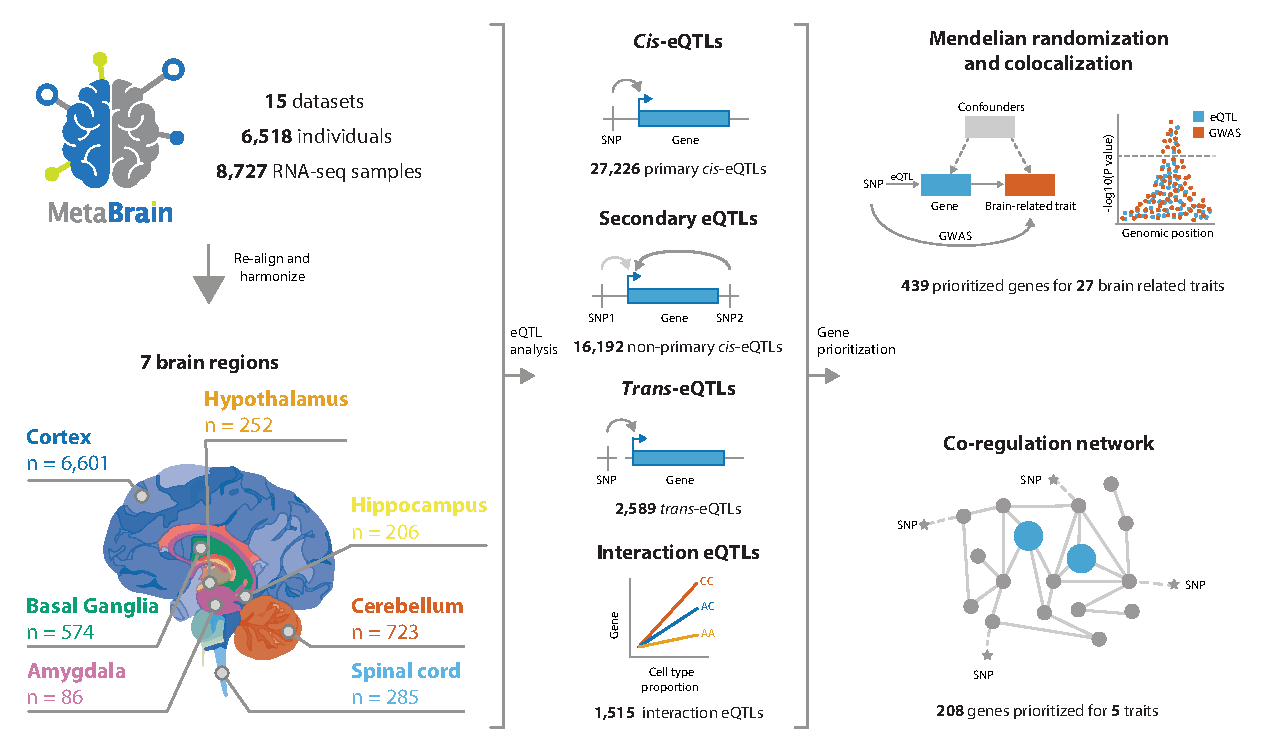
\includegraphics[width=\textwidth]{chapters/chapter5-brain-eqtls/img/2021-02-11-fig1-abstract_figure_v7.pdf}
	\caption{\textbf{Overview of the study.} We downloaded publicly available RNA-seq and genotype data from 15 different datasets consisting 8,727 RNA-seq measurements from 7 main brain regions in 6,518 individuals. We performed \textit{cis}-, \textit{trans}- and interaction-eQTL analysis, built a brain-specific gene coregulation network and prioritized genes using Mendelian randomization, colocalization and the co-regulation network.}
	\label{metabrain_fig1} 
\end{figure}


\Needspace{10\baselineskip}
\section{Results}
\Needspace{10\baselineskip}
\subsection{Leveraging public RNA-seq and genotype data to create large, harmonized brain eQTL and gene co-regulation datasets}
We combined 15 eQTL datasets into the ‘\textit{MetaBrain}’ resource to maximize statistical power to detect eQTLs, and to create a brain specific gene coregulation network (\textbf{Figure \ref{metabrain_fig2}; Supplementary table 1, Supplementary figures 1-5}). \textit{MetaBrain} includes 7,604 samples from the AMP-AD consortium\cite{hodesAcceleratingMedicinesPartnership2016} (AMP-AD MAYO\cite{hodesAcceleratingMedicinesPartnership2016}, ROSMAP\cite{hodesAcceleratingMedicinesPartnership2016} and MSBB\cite{hodesAcceleratingMedicinesPartnership2016}), Braineac\cite{ramasamyGeneticVariabilityRegulation2014}, the PsychENCODE consortium\cite{consortium*RevealingBrainMolecular2018} (Bipseq\cite{wangComprehensiveFunctionalGenomic2018}, BrainGVEX\cite{wangComprehensiveFunctionalGenomic2018}, CMC\cite{fromerGeneExpressionElucidates2016}, GVEX, and UCLA\_ASD\cite{wangComprehensiveFunctionalGenomic2018}), BrainSeq\cite{brainseq2015}, NABEC\cite{gibbsAbundantQuantitativeTrait2010}, TargetALS\cite{prudencioDistinctBrainTranscriptome2015}, and GTEx\cite{donovanCellularDeconvolutionGTEx2020}. Additionally, we carefully selected 1,759 brain RNA-seq samples from the European Nucleotide Archive (ENA)\cite{leinonenEuropeanNucleotideArchive2011}, calling and imputing genotypes based on the RNA-seq alignment (\textbf{Supplementary Note, Supplementary Figure 2-3}). Out of the 9,363 included RNA-seq samples, 8,727 remained after realignment and stringent quality control (\textbf{Supplementary Note}). We corrected the RNA-seq data for technical covariates, permitting us to define 7 major tissue groups (amygdala, basal ganglia, cerebellum, cortex, hippocampus, hypothalamus and spinal cord): PCA on the RNA-seq data showed clear clustering by these major tissue groups, resembling brain physiology (\textbf{Figure \ref{metabrain_fig2}D, Supplementary Figure 4}). Genotype data revealed individuals from different ethnicities (\textbf{Figure \ref{metabrain_fig2}B, Supplementary Figure 5}), including 5,138 samples from European descent (EUR), and 805 samples from African descent (AFR). Based on these sample characteristics, we created 7 eQTL discovery datasets: Basal ganglia-EUR (n=208), Cerebellum-EUR (n=492), Cortex-EUR (n=2,970), Cortex-AFR (n=420), Hippocampus-EUR (n=168) and Spinal cord-EUR (n=108; \textbf{Supplementary Table 1, Figure \ref{metabrain_fig2}C}). \emph{Cis}-eQTLs were not calculated for amygdala and hypothalamus tissue groups due to the small sample size (n$<$100). 

\begin{figure}[H]
	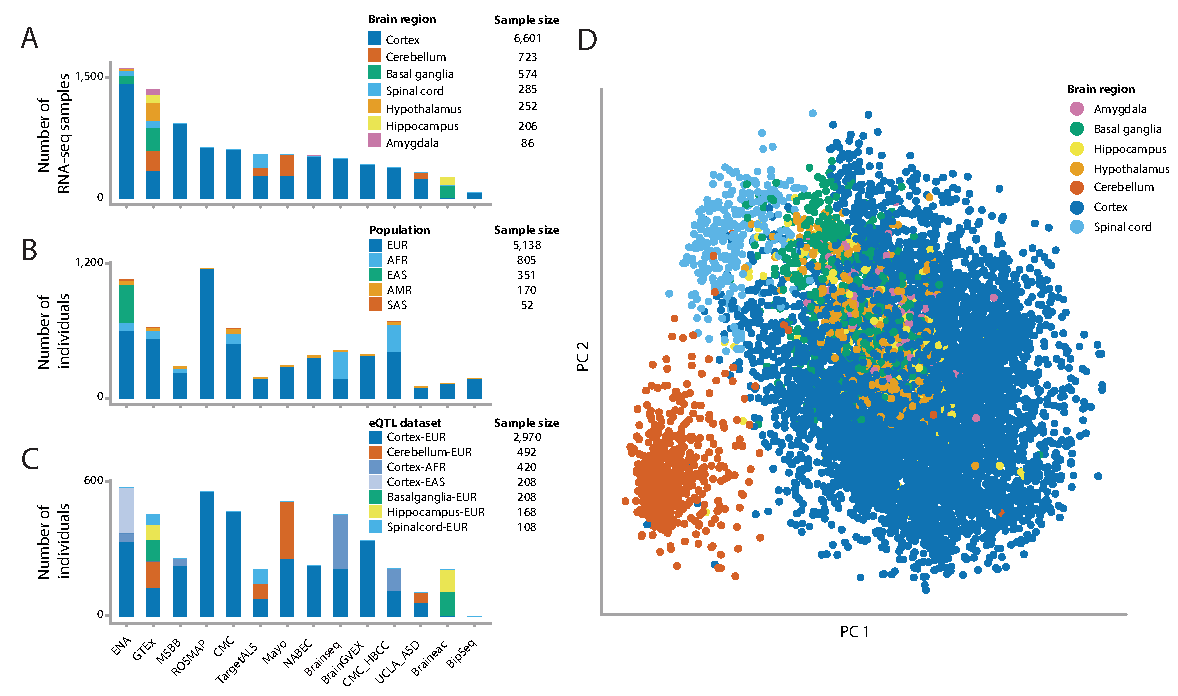
\includegraphics[width=\textwidth]{chapters/chapter5-brain-eqtls/img/2021-02-11-fig2-datasetoverview-v7.pdf}
	\caption{\textbf{Overview of the dataset.} \textbf{(A)} The number of samples per included cohort, with each color representing one of the 7 major brain regions. \textbf{(B)} The number of genotypes per cohort, with each color representing a population. \textbf{(C)} The number of individuals per cohort, with each color representing an eQTL dataset. The number of individuals is different from the intersection between the number of RNA-seq samples and number of genotypes, because not all samples with genotypes have RNA-seq samples and vice-versa, and some individuals with genotypes have multiple RNA-seq measurements. \textbf{(D)} PCA dimensionality reduction plot of the normalized expression data after covariate correction. Each dot represents a RNA-seq sample and is colored by brain region. The figure shows that the samples cluster mainly on brain region, and that is difficult to distinguish between cortex, hypothalamus, basal ganglia, and amygdala.}
	\label{metabrain_fig2}
\end{figure}

\Needspace{10\baselineskip}
\subsection{41\% of the cortex eQTL genes are regulated by multiple independent variants}
Within each discovery dataset, we performed a sample-size weighted \textit{cis}-eQTL meta-analysis on common variants (MAF$>$1\%), within 1 megabase (Mb) of the transcription start site (TSS) of a protein-coding gene. We identified 1,317 (Basal ganglia-EUR), 6,865 (Cerebellum-EUR), 5,440 (Cortex-AFR), 11,803 (Cortex-EUR), 990 (Hippocampus-EUR), and 811 (Spinal cord-EUR) \textit{cis}-eQTLs genes (FDR$<$0.05; \textbf{Figure \ref{metabrain_fig3}A; Supplementary Table 2}). eQTL effect directions were highly concordant between datasets included in the Cortex-EUR meta-analysis (Spearman r$>$0.59; allelic concordance$>$72\%; \textbf{Supplementary Figure 6}), indicating robustness of the identified effects across datasets. We noted that our alignment strategy excluded some \textit{cis}-eQTLs, such as the \textit{MAPT} locus (\textbf{Supplementary Note, Supplementary Figures 7-9}). We next performed conditional analysis to identify independent associations in each eQTL locus (e.g. secondary, tertiary and quaternary eQTLs). In Cortex-EUR, 4,791 genes had a significant secondary eQTL (41\% of \textit{cis}-eQTL genes identified in this dataset). 1,658 genes had tertiary and 598 had quaternary \textit{cis}-eQTLs. We also identified secondary associations for the other discovery datasets albeit to a lesser extent (\textbf{Figure \ref{metabrain_fig3}A, Supplementary Table 2 and 3}).  

The properties of the Cortex-EUR eQTLs conform to studies performed earlier in blood\cite{vosaUnravelingPolygenicArchitecture2018} and brain\cite{dobbynLandscapeConditionalEQTL2018} (\textbf{Figure \ref{metabrain_fig3}B}): primary lead \textit{cis}-eQTL SNPs were generally located close (median distance: 31 kilobase; kb) to the transcription start site (TSS; \textbf{Figure \ref{metabrain_fig3}B}) and were less likely linked to genes intolerant to loss of function mutations ($\chi^2$ $p = 6.35 \times 10^{-147}$). Genes with a \textit{cis}-eQTL generally had a higher median expression than those without (Wilcoxon p-value: $9.96 \times 10^{-12}$). Contrary to blood, where genes in the highest expression decile are the most likely to have a \textit{cis}-eQTL, the third decile of gene expression had the most \textit{cis}-eQTLs in cortex, and higher deciles had increasingly lower proportions of eQTLs (\textbf{Supplementary Note, Supplementary Figure 10A}). This could suggest that highly expressed brain genes in the cortex have tighter genetic regulation than highly expressed genes in the blood, although we did not observe difference when comparing vaereiance per gene expression decial between blood and brain (\textbf{Supplementary Note, Supplementary Figure 10B}). Cortex-EUR eQTL genes showed limited functional enrichment for human phenotype ontologies (HPO), GO ontologies and transcription factor motifs from TRANSFAC\cite{wingenderTRANSFACDatabaseTranscription1996} (\textbf{Supplementary Figure 10C and D, Supplementary Table 4}). We observed similar patterns for secondary, tertiary and quaternary eQTLs (\textbf{Supplementary Note}). 

We investigated differences in cis-eQTLs due to ancestry, brain region, data sets and tissue type. We compared Cortex-EUR, Cortex-AFR and a smaller, East Asian cortex dataset (Cortex-EAS; n=208, limited to the ENA cohort; \textbf{Figure \ref{metabrain_fig2}C}), and observed a high allelic concordance between the different ethnicities ($>$95.67\%; \textbf{Figure \ref{metabrain_fig3}C}). There was high concordance between different brain regions overall ($>$94.58\%), though the cerebellum showed lower concordance with the cerebral brain regions \textbf{Figure \ref{metabrain_fig3}D}. Despite the limited sample size compared to Cortex-EUR, we identified 846 \textit{cis}-eQTLs that were unique to Cerebellum-EUR (\textbf{Supplementary Figure 11A}). Of the 846 Cerebellum-EUR unique cis-eQTL genes, 184 had low gene expression levels in cortex, which may explain why they did not have a \textit{cis}-eQTL in that tissue(\textbf{Supplementary Figure 11B, C, Supplementary Note}). For the remaining 662 genes that were highly expressed in both cortex and cerebellum, we performed functional enrichment of transcription factor binding cites (TFBS; (\textbf{Supplementary Table 5, Supplementary Note}) and determined that these genes were enriched for TFBS of 101 distinct transcription faxtors. Five of these transcription factors had low gene expression in cortex  and high expression in cerebellum (\textit{EOMES}, \textit{TFAP2B}, \textit{TFAP2A}, \textit{IRX1} and \textit{IRX5}, \textbf{Supplementary Figure 11D}). These transcription factors might explain the difference in \textit{cis}-eQTL genes found in cerebellum but not in cortex, while many of these \textit{cis}-eQTL genes are expressed in both tissues. Next, we compared Cortex-EUR \textit{cis}-eQTLs with different tissues from the GTEx project (\textbf{Figure 3E; Supplementary Figure 12, Supplementary Table 6}). There was high concordance in brain-related tissues (cerebral tissues, $>$98\% and cerebellar tissues, $>$94\%) compared to other tissue types, and the lowest concordance rates were observed in testis (84\%) and whole blood (85\%). We also compared Cortex-EUR \textit{cis}-eQTLs with eQTLGen\cite{vosaUnravelingPolygenicArchitecture2018}, a large blood-based eQTL dataset (n=31,684; majority EUR ancestry) and observed a 76\% concordance rate (\textbf{Supplementary Figure 13; Supplementary Table 7}) with a moderate correlation of \textit{cis}-eQTL effect sizes (Rb=0.54 including all eQTLs, or Rb=0.62 when pruning genes within 1Mb)\cite{foleyFastEfficientColocalization2021}, supporting the lower concordance observed in GTEx-blood. Since we found that 24\% of the shared cis-eQTLs between blood and brain showed opposite allelic effects, these results suggest that with larger sample sizes, more tissue specific regulatory variants can be identified. If a causal tissue-specific regulatory variant resides on a haplotype that also contains a variant that is specific for another tissue, it is well conceivable that opposite allelic effects are going to be observed when contrasting eQTLs for these two tissues\cite{fuUnravelingRegulatoryMechanisms2012}. Since the procedures for eQTL mapping were identical between \textit{MetaBrain} and eQTLGen, our results highlight the relevance of tissue-specific eQTL mapping to accurately assess the directionality of eQTLs, which can elucidate eQTLs with opposite allelic effects\cite{fuUnravelingRegulatoryMechanisms2012}. This direct comparison illustrates the importance of investigating the appropriate tissue type for the interpretation of GWAS signals. 

\begin{sidewaysfigure}
	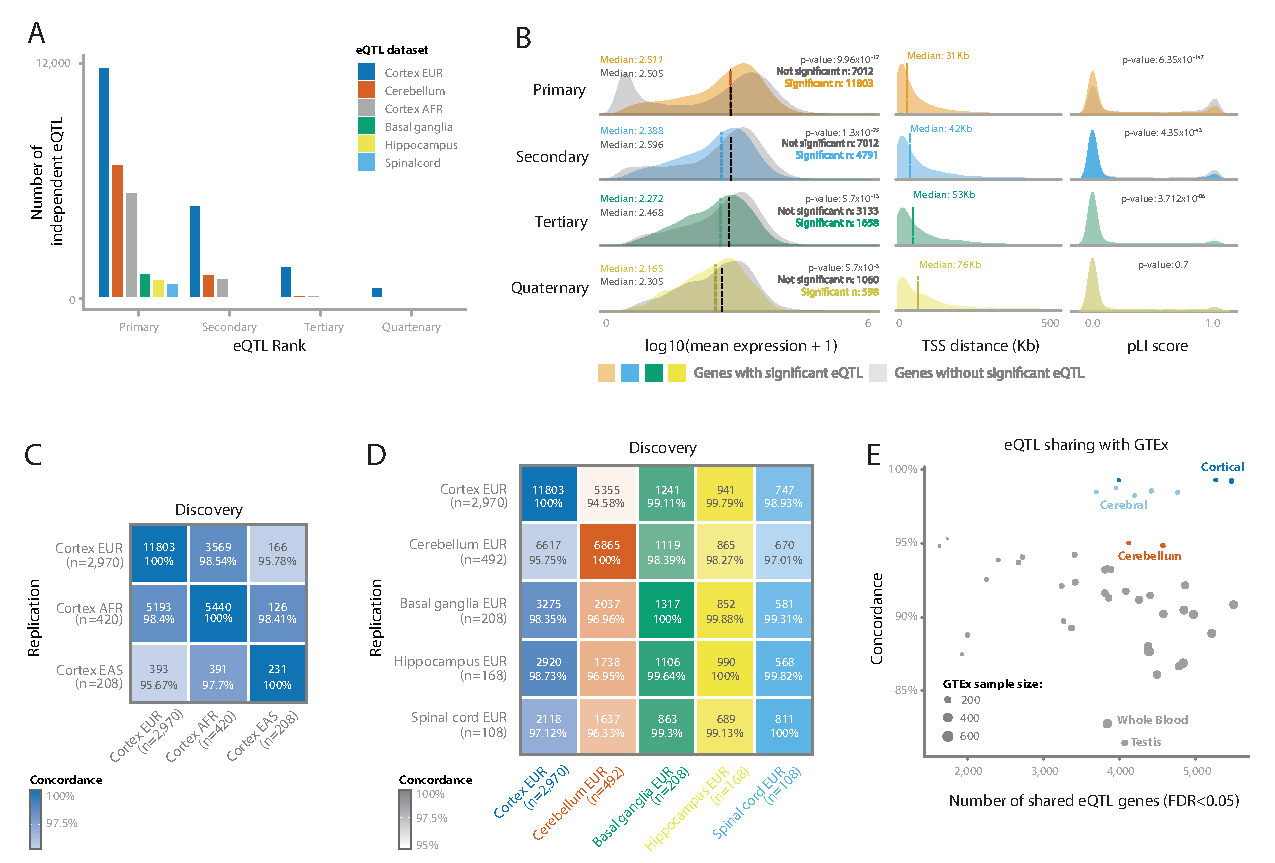
\includegraphics[width=\textwidth]{chapters/chapter5-brain-eqtls/img/2021-02-11-fig3-ciseqtls-v12.pdf}
	\caption{\textbf{Conditional \textit{cis}-eQTLs.} \textbf{(A)} The number of conditional \textit{cis}-eQTLs per eQTL dataset. \textbf{(B)} Comparison of characteristics between primary and non-primary eQTLs, for each plot the p-value is a wilcoxon test between significant and non-significant genes. (left) The difference in mean expression; (middle) the difference in distance between the most significant SNP-gene combination; (right) the difference in pLI score, for primary, secondary and quartenary eQTLs non-significnat eQTLs have higher pLI scores.  \textbf{(C, D)} Replication of primary \textit{cis}-eQTLs between; the cortex eQTLs of different ethnicities \textbf{(C)} and; \textbf{(D)} the different brain regions for the European datasets. The n under the dataset name is the number of samples in that dataset. The boxes show the number the number of eQTLs that are significant in both the discovery and the replication set, and the percentage of those that shows the same direction of effect. \textbf{(E)} The replication between primary \textit{cis}-eQTLs of Cortex-EUR (discovery) with all the GTEx tissues (replication). Each dot is a different GTEx tissue, the x-axis is the number of eQTLs that is significant in both discovery and replication, and the y-axis is the percentage that shows the same direction of effect. }
	\label{metabrain_fig3}
\end{sidewaysfigure}

\Needspace{10\baselineskip}
\subsection{8\% of Cortex \textit{cis}-eQTLs are mediated by cell type proportion differences  }
Cell type dependent eQTLs can be identified in bulk RNA-seq data by performing cell type deconvolution and determining cell type interaction eQTLs (ieQTLs)\cite{donovanCellularDeconvolutionGTEx2020,glastonburyCellTypeHeterogeneityAdipose2019,raulaguirregamboaDeconvolutionBulkBlood2020}. We predicted five major cell types using single cell RNA-seq derived signature profiles\cite{zhengyuCellMapCharacterizingType}. Of these, neurons were the most abundant cell type (median cell proportion: 32.8\%), followed by endothelial cells (24.9\%), macrophages (17.8\%), oligodendrocytes (12.4\%), astrocytes (12.1\%; \textbf{Supplementary Figure 14}). We predicted similar proportions for cerebellum as well as other brain regions. We observed that predicted cell proportions are different for spinal cord, showing a relatively low proportion of neuronal cells and high proportions of macrophage and oligodendrocytes compared to other brain tissues, as was previously reported\cite{bahneyCellularCompositionGliaNeuron2018} (\textbf{Supplementary Figures 15 and 16}). Predicted neuron proportions in both cortex and cerebellum were negatively correlated with the predicted proportions of other cell types, and predicted endothelial cell proportions were negatively correlated with predicted macrophage proportions (\textbf{Figure \ref{metabrain_fig4}A}). Predicted cell type proportions were positively correlated with immunochemistry (IHC) counts from the ROSMAP cohort\cite{patrickDeconvolvingContributionsCelltype2020}, both overall (Spearman r = 0.71; \textbf{\ref{metabrain_fig4}B}), and per individual cell type (Spearman r$>$0.1; \textbf{\ref{metabrain_fig4}}).  It is difficult to validate these cell type proportion predictions due to the small scale of the IHC experiment, but also because IHC and bulk RNA-seq reflect different aspects of gene or protein expression. Thus, there is a level of uncertainty for the expected proportion for each cell type\cite{herculano-houzelHumanBrainNumbers2009,vonbartheldSearchTrueNumbers2016}. 

With these predicted cell type proportions, we used DeconQTL\cite{raulaguirregamboaDeconvolutionBulkBlood2020} to identify interaction-eQTLs (ieQTLs) by testing 18,850 \textit{cis}-eQTLs in Cortex-EUR and 8,347 \textit{cis}-eQTLs in cerebellum (including primary, secondary, tertiary and quaternary eQTLs). We identified 1,515 significant ieQTLs (8\%) in at least one cell type (Benjamini-Hochberg; BH FDR $<$ 0.05) for Cortex-EUR (\textbf{Supplementary Table 8}). Of these, 632 (42\%) were an ieQTL in neurons, likely because this is the most prevalent cell type. The majority (90.2\%) of the ieQTLs were uniquely mapped to one cell type (\textbf{Figure \ref{metabrain_fig4}C}).Although we observed a lower proportion of ieQTLs in cerebellum (126; 1.5\%, \textbf{Supplementary Figure 17, Supplementary Table 8}), this is likely a power issue due to the smaller sample size. While we observed most ieQTLs for neurons in cortex, the majority (n=106; 84\%) of these ieQTLs were mediated by astrocytes and macrophages.  

We compared the allelic direction of the identified ieQTLs for each cell type with matching cell types from a single nucleus RNA-seq (snRNA-seq) dataset (ROSMAP cohort, n=39; \textbf{Supplementary Table 9})\cite{mathysSinglecellTranscriptomicAnalysis2019}. When filtering on cell-type mediated eQTLs by Decon-QTL (FDR $<$ 0.05) we observed a high average concordance in allelic direction for both the eQTL main effect (68\%), as well as the direction of the interaction (68\%; \textbf{Supplementary Figure 18B}). 106 of the cortex \textit{cis}-ieQTLs were also significant (BH FDR$<$0.05) in the snRNA-seq datasets (63 in excitatory neurons and 43 in oligodendrocytes). Of these, 13 excitatory neuron and 21 oligodendrocyte ieQTLs were cell type mediated by the corresponding cell type in bulk (Decon-QTL; BH FDR $<$ 0.05; \textbf{Supplementary Figure 18D}). The ieQTLs replicating in oligodendrocytes included \textit{STMN4}, \textit{NKAIN1}, and \textit{FAM221A} (\textbf{Figure \ref{metabrain_fig4}D and E and Supplementary Figure 19A-C}), which have previously been identified as oligodendrocyte specific\cite{ngUsingTranscriptomicHidden2019}. Additionally, this set of ieQTLs included \textit{AMPD3} (rs11042811) and \textit{CD82} (rs2303865), genes involved in white matter microstructure\cite{zhaoLargescaleGWASReveals2019}, suggesting a role for oligodendrocytes in this pathway. The ieQTLs replicating in excitatory neurons included \textit{SLC25A27} (alias \textit{UCP4}; \textbf{4F and Supplementary Figure 19D}), a gene principally expressed in neurons\cite{smorodchenkoComparativeAnalysisUncoupling2009} that modulates neuronal metabolism\cite{liuMitochondrialUCP4Mediates2006}. The eQTL SNP for this gene, rs2270450, is in high LD ($R^2$=0.71) with a variant previously associated with schizophrenia\cite{yasunoSynergisticAssociationMitochondrial2007}. Previous work has suggested a possible role of this gene in Parkinson’s disease\cite{ramsdenHumanNeuronalUncoupling2012,hoMitochondrialNeuronalUncoupling2012}. These results suggest that the decomposition of eQTLs to their relevant cell types in \textit{MetaBrain} yields additional valuable information about the underlying biological mechanisms of genes and cell types of interest for genes associated with disease.

\begin{figure}[H]
	\includegraphics[width=\textwidth]{chapters/chapter5-brain-eqtls/img/2021-02-11-fig4-interactionqtls-v11.pdf}
	\caption{\textbf{Cell type interacting eQTLs.} \textbf{(A)} Spearman correlations between the 5 predicted cell count proportions. Lower triangle is within cortex samples, upper triangle is within cerebellum samples. \textbf{(B)} Predicted cell count proportions (x-axis) compared to measured cell count proportions (y-axis) for 42 ROSMAP samples. Values in the plot are Pearson correlation coefficients. Cell count predictions for most cells closely approximates actual IHC cell counts., although neurons tend to be underestimated. (C) Number of cell type interacting eQTLs for Cortex-EUR deconvoluted cell types. The majority of interactions are with neurons and oligodendrocytes. Notably, most interactions are unique for one cell type in 95\% of the cases. \textbf{(D, E, F)} Replication of cell type interacting eQTLs for STMN4 \textbf{(D)}, FAM221A \textbf{(E)} and SLC25A27 \textbf{(F)}. Left; scatterplot of the interaction eQTL in \textit{MetaBrain}  bulk RNA-seq. The x-axis shows the estimated cell type proportion, the y-axis shows the gene expression, each dot represents a sample and the colors are according to the SNP genotype. Values in the plot are Spearman correlation coefficients. Right; forest plot of the spearman coefficient when replicating the eQTL effect in ROSMAP single nucleus data. The error bar is calculated based on the results of Bonett and Wright\cite{bonettSampleSizeRequirements2000}. Each row denotes a cell type specific dataset: excitatory neurons (EX), oligodendrocytes (OLI), inhibitory neurons (IN), astrocytes (AST), oligodendrocyte precursor cells (OPC), microglia (MIC), pericytes (PER) and endothelial cells (END). The bold cell type corresponds to the cell type estimated on the left figure. }
	\label{metabrain_fig4}
\end{figure}

\Needspace{10\baselineskip}
\subsection{Shared genetic effects between Cortex-EUR \textit{cis}-eQTLs and brain-related traits}

As one application of the \textit{MetaBrain} resource, we linked \textit{cis}-eQTLs to variants associated with neurological traits and diseases. For this, we first evaluated linkage disequilibrium (LD) between the Cortex-EUR \textit{cis}-eQTL SNPs with the strongest association signals and index variants identified in 3,217 GWASs of brain-related traits (\textbf{Supplementary Note, Supplementary Table 10}). We observed that 10\% of brain-related trait SNPs for 242 eQTL genes were in LD with \textit{cis}-eQTL SNPs (r2$>$0.8). This percentage marginally increased to 12\% when secondary, tertiary and quaternary eQTL SNPs were included, indicating that the majority of LD overlap is driven by primary eQTL effects: primary eQTLs were 3.3-fold more likely to be in LD with a GWAS SNP (Fisher exact test p-value = $6.2 \times 10^{-16}$; \textbf{Supplementary Note}). 

To more formally test for overlap between GWAS and eQTL signals, we next implemented a Mendelian Randomization (MR) analysis to test for a causal effect between gene expression and 31 neurological traits using \textit{cis}-eQTLs as instruments (\textbf{Supplementary Table 11}). We computed a Wald ratio for each eQTL instrument, from which 1,192 Wald ratios out of 268,030 tested in total passed our suggestive p-value threshold ($p<5 \times 10^{-5}$; \textbf{Supplementary Table 12}). 120 of the cis-eQTL instruments from these suggestive findings were also cell type ieQTLs. We further prioritized our list of genes with evidence of Wald ratio effects by determining genetic colocalization between GWAS and \textit{cis}-eQTL signals using COLOC\cite{deelenGenotypeHarmonizerAutomatic2014}. There were 159 significant Wald ratios that passed a strict Bonferroni correction ($p<1.87 \times 10^{-7}$) where the GWAS SNP and eQTL colocalized (PP4$>$0.7; \textbf{Figure \ref{metabrain_fig5}A; Supplementary Figure 20}). 69 of these prioritized findings were associated with neurological and neuropsychiatric disease risk (\textbf{Table \ref{metabrain_tab1}}). Three examples where MR and colocalization pointed to likely causal GWAS genes are reported below, for others, see \textbf{Supplementary Note, Supplementary Tables 11-16 and Supplementary Figures 21 and 22}.

% Table was generate using https://www.tablesgenerator.com/
\begin{table}[]
	\centering
	\caption{\textbf{Prioritized genes from the Mendelian Randomization analysis on MetaBrain eQTLs versus brain related outcomes.} Harmonized eQTL and GWAS SNP effects and single SNP Wald Ratio estimates are reported in the table for all genes with Wald Ratio effects at $P < 1.865 \times 10^{-7}$.}
	\label{metabrain_tab1}
	\resizebox{\textwidth}{!}{
	\begin{tabular}{llllllllllll}
		& \multicolumn{4}{c}{\cellcolor[HTML]{00B050}{\color{white}MetaBrain eQTL instrument}}  & \multicolumn{4}{c}{\cellcolor[HTML]{4472C4}{\color{white}Brain-related trait outcome SNP effects}}   & \multicolumn{3}{c}{\cellcolor[HTML]{ff8c00 }{\color{white}MR effects}}  \\
		\multicolumn{1}{c}{\textbf{SNP}} & \multicolumn{1}{c}{\textbf{gene}} & \multicolumn{1}{c}{\textbf{beta}} & \multicolumn{1}{c}{\textbf{SE}} & \multicolumn{1}{c}{\textbf{p}} & \multicolumn{1}{c}{\textbf{outcome}}       & \multicolumn{1}{c}{\textbf{beta}} & \multicolumn{1}{c}{\textbf{SE}} & \multicolumn{1}{c}{\textbf{p}} & \multicolumn{1}{c}{\textbf{WR}} & \multicolumn{1}{c}{\textbf{SE}} & \multicolumn{1}{c}{\textbf{p}} \\
		\rowcolor[HTML]{E0E0E0}rs679515:T/C                     & CR1                               & 0.824                             & 0.032                           & 2.45E-145                      & Alzheimer’s disease                        & 0.123                             & 0.012                           & 1.40E-23                       & 0.149                           & 0.015                           & 1.40E-23                       \\
		\rowcolor[HTML]{E0E0E0}rs6069736:T/C                    & CASS4                             & 0.252                             & 0.044                           & 9.43E-09                       & Alzheimer’s disease                        & -0.105                            & 0.017                           & 6.52E-10                       & -0.415                          & 0.067                           & 6.52E-10                       \\
		\rowcolor[HTML]{E0E0E0}rs10749609:G/A                   & TSPAN14                           & -0.398                            & 0.034                           & 1.37E-31                       & Alzheimer’s disease                        & -0.068                            & 0.012                           & 6.71E-09                       & 0.171                           & 0.030                           & 6.71E-09                       \\
		\rowcolor[HTML]{E0E0E0}rs55667375:T/C                   & PRSS36                            & 0.578                             & 0.027                           & 8.28E-101                      & Alzheimer’s disease                        & -0.061                            & 0.011                           & 1.74E-08                       & -0.105                          & 0.019                           & 1.74E-08                       \\
		\rowcolor[HTML]{E0E0E0}rs7196161:G/A                    & ZNF668                            & 0.150                             & 0.026                           & 1.19E-08                       & Alzheimer’s disease                        & 0.053                             & 0.010                           & 5.48E-08                       & 0.354                           & 0.065                           & 5.48E-08                       \\
		\rowcolor[HTML]{E0E0E0}rs1171830:C/A                    & CCDC6                             & 0.165                             & 0.026                           & 1.75E-10                       & Alzheimer’s disease                        & 0.051                             & 0.010                           & 8.60E-08                       & 0.311                           & 0.058                           & 8.60E-08                       \\
		\rowcolor[HTML]{E0E0E0}rs75763893:T/C                   & APH1B                             & 0.354                             & 0.039                           & 1.51E-19                       & Alzheimer’s disease                        & 0.080                             & 0.015                           & 9.52E-08                       & 0.226                           & 0.042                           & 9.52E-08                       \\
		\rowcolor[HTML]{E0E0E0}	rs749671:A/G                     & ZNF646                            & -0.190                            & 0.026                           & 1.96E-13                       & Alzheimer’s disease                        & 0.052                             & 0.010                           & 1.00E-07                       & -0.273                          & 0.051                           & 1.00E-07                       \\
		\rowcolor[HTML]{E0E0E0}rs2855475:G/A                    & KAT8                              & -0.334                            & 0.026                           & 2.33E-38                       & Alzheimer’s disease                        & 0.052                             & 0.010                           & 1.11E-07                       & -0.156                          & 0.029                           & 1.11E-07                       \\
		\rowcolor[HTML]{E0E0E0}rs4291:T/A                       & ACE                               & 0.340                             & 0.028                           & 1.09E-34                       & Alzheimer’s disease                        & -0.052                            & 0.010                           & 1.39E-07                       & -0.153                          & 0.029                           & 1.39E-07                       \\
		\rowcolor[HTML]{BEBEBE}rs2045180:A/G                    & G2E3                              & -0.269                            & 0.027                           & 2.79E-23                       & Amyotrophic Lateral Sclerosis              & 0.092                             & 0.012                           & 5.70E-15                       & -0.343                          & 0.044                           & 5.56E-15                       \\
		\rowcolor[HTML]{BEBEBE}rs229243:A/C                     & SCFD1                             & 0.397                             & 0.027                           & 1.14E-50                       & Amyotrophic Lateral Sclerosis              & 0.092                             & 0.012                           & 5.41E-15                       & 0.232                           & 0.030                           & 5.56E-15                       \\
		\rowcolor[HTML]{E0E0E0}rs9834970:C/T                    & DCLK3                             & -0.189                            & 0.026                           & 1.99E-13                       & Bipolar disorder                           & 0.101                             & 0.013                           & 5.53E-14                       & -0.534                          & 0.071                           & 4.79E-14                       \\
		\rowcolor[HTML]{E0E0E0}rs55762233:G/C                   & HAPLN4                            & 0.317                             & 0.034                           & 3.70E-21                       & Bipolar disorder                           & 0.106                             & 0.018                           & 3.20E-09                       & 0.335                           & 0.057                           & 3.07E-09                       \\
		\rowcolor[HTML]{E0E0E0}rs7646741:G/A                    & GNL3                              & -0.225                            & 0.026                           & 1.82E-18                       & Bipolar disorder                           & -0.077                            & 0.014                           & 9.52E-09                       & 0.343                           & 0.060                           & 1.07E-08                       \\
		\rowcolor[HTML]{E0E0E0}rs2271893:A/G                    & LMAN2L                            & 0.255                             & 0.028                           & 8.72E-20                       & Bipolar disorder                           & -0.081                            & 0.014                           & 2.08E-08                       & -0.317                          & 0.056                           & 1.93E-08                       \\
		\rowcolor[HTML]{E0E0E0}rs113980591:A/G                  & CILP2                             & 0.185                             & 0.033                           & 3.46E-08                       & Bipolar disorder                           & 0.097                             & 0.018                           & 3.65E-08                       & 0.525                           & 0.095                           & 3.68E-08                       \\
		\rowcolor[HTML]{E0E0E0}rs8102502:C/T                    & TM6SF2                            & 0.254                             & 0.032                           & 3.54E-15                       & Bipolar disorder                           & 0.092                             & 0.017                           & 9.50E-08                       & 0.361                           & 0.068                           & 9.75E-08                       \\
		\rowcolor[HTML]{BEBEBE}rs2815764:A/G                    & NEGR1                             & -0.269                            & 0.036                           & 1.16E-13                       & Depression (broad)                         & -0.008                            & 0.001                           & 3.74E-08                       & 0.030                           & 0.006                           & 3.74E-08                       \\
		\rowcolor[HTML]{BEBEBE}rs4578918:T/C                    & SLC12A5                           & 0.181                             & 0.029                           & 5.13E-10                       & Depression (broad)                         & 0.007                             & 0.001                           & 8.72E-08                       & 0.040                           & 0.007                           & 8.71E-08                       \\
		\rowcolor[HTML]{E0E0E0}rs9268863:A/G                    & BTNL2                             & 0.365                             & 0.026                           & 9.05E-45                       & Frontotemporal Dementia                    & 0.279                             & 0.044                           & 2.20E-10                       & 0.764                           & 0.120                           & 2.20E-10                       \\
		\rowcolor[HTML]{BEBEBE}rs4794333:C/T                    & CDK5RAP3                          & 0.351                             & 0.026                           & 1.42E-42                       & Generalized epilepsy, all documented cases & -0.074                            & 0.013                           & 6.81E-09                       & -0.210                          & 0.036                           & 6.79E-09                       \\
		\rowcolor[HTML]{E0E0E0}rs11150600:C/T                   & HSD3B7                            & 0.174                             & 0.027                           & 1.60E-10                       & Juvenile myoclonic epilepsy                & 0.011                             & 0.002                           & 4.00E-09                       & 0.065                           & 0.011                           & 3.96E-09                       \\
		\rowcolor[HTML]{BEBEBE}rs9970196:T/C                    & TTC34                             & 0.284                             & 0.027                           & 1.10E-25                       & Multiple sclerosis                         & -0.145                            & 0.018                           & 2.04E-15                       & -0.511                          & 0.064                           & 2.04E-15                       \\
		\rowcolor[HTML]{BEBEBE}rs28895017:A/C                   & HLA-DRB1                          & -0.652                            & 0.089                           & 1.88E-13                       & Multiple sclerosis                         & -0.530                            & 0.072                           & 1.41E-13                       & 0.814                           & 0.110                           & 1.41E-13                       \\
		\rowcolor[HTML]{BEBEBE}rs62120372:A/T                   & MPV17L2                           & 0.168                             & 0.029                           & 4.76E-09                       & Multiple sclerosis                         & -0.132                            & 0.019                           & 1.28E-12                       & -0.790                          & 0.111                           & 1.29E-12                       \\
		\rowcolor[HTML]{BEBEBE}rs4578918:T/C                    & SLC12A5                           & 0.181                             & 0.029                           & 5.13E-10                       & Multiple sclerosis                         & 0.129                             & 0.018                           & 1.89E-12                       & 0.711                           & 0.101                           & 1.89E-12                       \\
		\rowcolor[HTML]{BEBEBE}rs10877011:G/T                   & EEF1AKMT3                         & 0.775                             & 0.024                           & 1.00E-200                      & Multiple sclerosis                         & -0.116                            & 0.018                           & 5.13E-11                       & -0.150                          & 0.023                           & 5.13E-11                       \\
		\rowcolor[HTML]{BEBEBE}rs11172335:T/C                   & TSFM                              & -0.547                            & 0.026                           & 3.59E-98                       & Multiple sclerosis                         & -0.113                            & 0.018                           & 1.57E-10                       & 0.207                           & 0.032                           & 1.57E-10                       \\
		\rowcolor[HTML]{BEBEBE}rs4794007:G/A                    & NPEPPS                            & -0.174                            & 0.026                           & 1.75E-11                       & Multiple sclerosis                         & -0.107                            & 0.017                           & 2.98E-10                       & 0.618                           & 0.098                           & 2.97E-10                       \\
		\rowcolor[HTML]{BEBEBE}rs2288481:A/G                    & CCDC155                           & -0.193                            & 0.033                           & 4.83E-09                       & Multiple sclerosis                         & 0.119                             & 0.020                           & 9.33E-10                       & -0.620                          & 0.101                           & 9.33E-10                       \\
		\rowcolor[HTML]{BEBEBE}rs7306304:A/G                    & CLECL1                            & -0.604                            & 0.025                           & 6.52E-130                      & Multiple sclerosis                         & 0.098                             & 0.016                           & 1.58E-09                       & -0.162                          & 0.027                           & 1.58E-09                       \\
		\rowcolor[HTML]{BEBEBE}rs2259735:C/T                    & CYP24A1                           & -0.824                            & 0.023                           & 1.00E-200                      & Multiple sclerosis                         & -0.104                            & 0.017                           & 1.67E-09                       & 0.126                           & 0.021                           & 1.67E-09                       \\
		\rowcolor[HTML]{BEBEBE}rs10877023:A/C                   & TSPAN31                           & -0.166                            & 0.029                           & 7.62E-09                       & Multiple sclerosis                         & -0.108                            & 0.018                           & 1.73E-09                       & 0.655                           & 0.109                           & 1.73E-09                       \\
		\rowcolor[HTML]{BEBEBE}rs180534:C/T                     & RNFT1                             & -0.274                            & 0.026                           & 1.59E-26                       & Multiple sclerosis                         & 0.097                             & 0.016                           & 2.14E-09                       & -0.355                          & 0.059                           & 2.14E-09                       \\
		\rowcolor[HTML]{BEBEBE}rs9783665:T/A                    & TRAF3                             & 0.262                             & 0.027                           & 1.55E-22                       & Multiple sclerosis                         & 0.097                             & 0.017                           & 1.04E-08                       & 0.371                           & 0.065                           & 1.03E-08                       \\
		\rowcolor[HTML]{BEBEBE}rs6980663:C/G                    & IL7                               & -0.604                            & 0.027                           & 2.47E-113                      & Multiple sclerosis                         & 0.102                             & 0.018                           & 1.74E-08                       & -0.169                          & 0.030                           & 1.74E-08                       \\
		\rowcolor[HTML]{BEBEBE}rs6421983:T/C                    & IFITM1                            & 0.320                             & 0.026                           & 1.01E-33                       & Multiple sclerosis                         & 0.158                             & 0.028                           & 1.78E-08                       & 0.495                           & 0.088                           & 1.78E-08                       \\
		\rowcolor[HTML]{BEBEBE}rs34481144:T/C                   & IFITM3                            & -0.358                            & 0.026                           & 2.07E-42                       & Multiple sclerosis                         & 0.158                             & 0.028                           & 2.34E-08                       & -0.440                          & 0.079                           & 2.34E-08                       \\
		\rowcolor[HTML]{BEBEBE}rs3809627:A/C                    & TBX6                              & -0.428                            & 0.025                           & 2.07E-65                       & Multiple sclerosis                         & -0.097                            & 0.018                           & 3.25E-08                       & 0.226                           & 0.041                           & 3.25E-08                       \\
		\rowcolor[HTML]{BEBEBE}rs131813:A/G                     & SCO2                              & 0.221                             & 0.031                           & 5.21E-13                       & Multiple sclerosis                         & 0.109                             & 0.020                           & 6.20E-08                       & 0.493                           & 0.091                           & 6.20E-08                       \\
		\rowcolor[HTML]{BEBEBE}rs9866116:G/A                    & MYNN                              & 0.182                             & 0.031                           & 4.00E-09                       & Multiple sclerosis                         & -0.101                            & 0.019                           & 1.22E-07                       & -0.557                          & 0.105                           & 1.22E-07                       \\
		\rowcolor[HTML]{BEBEBE}rs4796224:G/A                    & MYO19                             & 0.331                             & 0.025                           & 3.02E-39                       & Multiple sclerosis                         & 0.085                             & 0.016                           & 1.62E-07                       & 0.258                           & 0.049                           & 1.62E-07                       \\
		\rowcolor[HTML]{E0E0E0}rs1724390:A/C                    & LRRC37A2                          & 0.957                             & 0.028                           & 1.00E-200                      & Parkinson’s disease                        & -0.210                            & 0.026                           & 5.00E-16                       & -0.219                          & 0.027                           & 5.14E-16                       \\
		\rowcolor[HTML]{E0E0E0}rs11724635:C/A                   & CD38                              & 0.424                             & 0.025                           & 5.84E-65                       & Parkinson’s disease                        & -0.125                            & 0.017                           & 1.23E-13                       & -0.294                          & 0.040                           & 1.20E-13                       \\
		\rowcolor[HTML]{E0E0E0}rs11150600:C/T                   & HSD3B7                            & 0.174                             & 0.027                           & 1.60E-10                       & Parkinson’s disease                        & -0.117                            & 0.018                           & 1.93E-10                       & -0.675                          & 0.106                           & 1.90E-10                       \\
		\rowcolor[HTML]{E0E0E0}rs823118:C/T                     & RAB29                             & -0.345                            & 0.026                           & 3.51E-41                       & Parkinson’s disease                        & -0.100                            & 0.017                           & 4.94E-09                       & 0.290                           & 0.050                           & 5.15E-09                       \\
		\rowcolor[HTML]{E0E0E0}rs11547135:T/C                   & SCARB2                            & 0.261                             & 0.027                           & 5.35E-22                       & Parkinson’s disease                        & 0.100                             & 0.018                           & 1.66E-08                       & 0.382                           & 0.068                           & 1.77E-08                       \\
		\rowcolor[HTML]{E0E0E0}rs199348:A/C                     & GPNMB                             & -0.827                            & 0.022                           & 1.00E-200                      & Parkinson’s disease                        & -0.098                            & 0.018                           & 2.31E-08                       & 0.119                           & 0.021                           & 2.26E-08                       \\
		\rowcolor[HTML]{BEBEBE}rs693906:C/G                     & CLIC1                             & -0.301                            & 0.037                           & 7.34E-16                       & Schizophrenia                              & -0.142                            & 0.016                           & 1.09E-18                       & 0.473                           & 0.054                           & 9.70E-19                       \\
		\rowcolor[HTML]{BEBEBE}rs2949006:T/G                    & FTCDNL1                           & -0.507                            & 0.032                           & 1.87E-56                       & Schizophrenia                              & 0.103                             & 0.014                           & 6.67E-14                       & -0.203                          & 0.027                           & 7.97E-14                       \\
		\rowcolor[HTML]{BEBEBE}rs4702:G/A                       & FURIN                             & -0.220                            & 0.026                           & 1.49E-17                       & Schizophrenia                              & 0.081                             & 0.012                           & 2.62E-12                       & -0.367                          & 0.052                           & 2.55E-12                       \\
		\rowcolor[HTML]{BEBEBE}rs2565161:C/G                    & SF3B1                             & 0.256                             & 0.027                           & 8.20E-21                       & Schizophrenia                              & 0.075                             & 0.012                           & 7.52E-11                       & 0.292                           & 0.045                           & 7.80E-11                       \\
		\rowcolor[HTML]{BEBEBE}rs55970317:G/T                   & PCCB                              & 0.339                             & 0.026                           & 2.74E-39                       & Schizophrenia                              & -0.070                            & 0.011                           & 1.92E-10                       & -0.207                          & 0.032                           & 1.75E-10                       \\
		\rowcolor[HTML]{BEBEBE}rs151022560:T/C                  & CNTN4                             & 0.223                             & 0.038                           & 3.36E-09                       & Schizophrenia                              & 0.095                             & 0.015                           & 2.39E-10                       & 0.428                           & 0.068                           & 2.65E-10                       \\
		\rowcolor[HTML]{BEBEBE}rs9834970:C/T                    & DCLK3                             & -0.189                            & 0.026                           & 1.99E-13                       & Schizophrenia                              & 0.067                             & 0.011                           & 6.35E-10                       & -0.354                          & 0.057                           & 5.53E-10                       \\
		\rowcolor[HTML]{BEBEBE}rs11038914:T/C                   & MDK                               & -0.219                            & 0.034                           & 8.78E-11                       & Schizophrenia                              & 0.089                             & 0.014                           & 5.99E-10                       & -0.404                          & 0.065                           & 5.81E-10                       \\
		\rowcolor[HTML]{BEBEBE}rs832190:C/T                     & THOC7                             & -0.291                            & 0.026                           & 2.49E-28                       & Schizophrenia                              & 0.070                             & 0.011                           & 5.73E-10                       & -0.240                          & 0.039                           & 6.19E-10                       \\
		\rowcolor[HTML]{BEBEBE}rs6224:T/G                       & FES                               & -0.246                            & 0.026                           & 9.65E-22                       & Schizophrenia                              & -0.068                            & 0.011                           & 8.37E-10                       & 0.278                           & 0.045                           & 7.19E-10                       \\
		\rowcolor[HTML]{BEBEBE}rs7957096:A/G                    & KMT5A                             & -0.170                            & 0.028                           & 1.40E-09                       & Schizophrenia                              & 0.071                             & 0.012                           & 1.52E-09                       & -0.418                          & 0.069                           & 1.69E-09                       \\
		\rowcolor[HTML]{BEBEBE}rs9925915:C/G                    & INO80E                            & -0.380                            & 0.025                           & 1.25E-51                       & Schizophrenia                              & -0.065                            & 0.011                           & 1.88E-09                       & 0.172                           & 0.029                           & 1.87E-09                       \\
		\rowcolor[HTML]{BEBEBE}rs7646741:G/A                    & GNL3                              & -0.225                            & 0.026                           & 1.82E-18                       & Schizophrenia                              & -0.064                            & 0.011                           & 3.78E-09                       & 0.286                           & 0.048                           & 3.46E-09                       \\
		\rowcolor[HTML]{BEBEBE}rs79235996:T/C                   & RGS6                              & -0.219                            & 0.038                           & 6.71E-09                       & Schizophrenia                              & 0.080                             & 0.014                           & 1.58E-08                       & -0.367                          & 0.065                           & 1.63E-08                       \\
		\rowcolor[HTML]{BEBEBE}rs2965183:A/G                    & GATAD2A                           & -0.416                            & 0.026                           & 1.44E-57                       & Schizophrenia                              & 0.064                             & 0.011                           & 1.68E-08                       & -0.153                          & 0.027                           & 1.82E-08                       \\
	\rowcolor[HTML]{BEBEBE}	rs1763839:A/G                    & RERE                              & 0.229                             & 0.028                           & 3.70E-16                       & Schizophrenia                              & 0.064                             & 0.012                           & 2.37E-08                       & 0.281                           & 0.050                           & 2.14E-08                       \\
	\rowcolor[HTML]{BEBEBE}	rs72986630:`/C                   & ZNF823                            & 0.654                             & 0.054                           & 1.85E-33                       & Schizophrenia                              & 0.146                             & 0.027                           & 4.12E-08                       & 0.223                           & 0.041                           & 4.14E-08                       \\
		\rowcolor[HTML]{BEBEBE}rs6445358:C/G                    & GLYCTK                            & 0.229                             & 0.026                           & 4.87E-19                       & Schizophrenia                              & 0.059                             & 0.011                           & 6.74E-08                       & 0.257                           & 0.048                           & 7.22E-08                       \\
		\rowcolor[HTML]{BEBEBE}rs10520163:T/C                   & CLCN3                             & 0.160                             & 0.026                           & 4.94E-10                       & Schizophrenia                              & 0.058                             & 0.011                           & 7.36E-08                       & 0.364                           & 0.068                           & 8.03E-08                       \\
		\rowcolor[HTML]{BEBEBE}rs1009136:A/G                    & MAU2                              & -0.277                            & 0.027                           & 8.07E-25                       & Schizophrenia                              & 0.060                             & 0.011                           & 1.37E-07                       & -0.217                          & 0.041                           & 1.35E-07                      
	\end{tabular}}
\end{table}

\Needspace{10\baselineskip}
\subsection{MR comparison between blood and brain eQTL datasets}
MR analysis for multiple sclerosis (MS) identified 157 instruments that passed the suggestive threshold of $p<5 \times 10^{-5}$, representing 135 unique genes (\textbf{Supplementary Table 12}). 20 of these findings passed colocalization (\textbf{Table 1; Figure \ref{metabrain_fig5}B}). This included 11 genes for which MR suggested that increased gene expression and 9 genes where decreased gene expression leads to MS risk. Systematic comparison of the MR Wald ratio estimates for MS of 5,919 shared eQTL genes between Cortex-EUR and eQTLGen\cite{vosaUnravelingPolygenicArchitecture2018} (where the same gene was instrumented but could be with different SNPs) showed opposite directions of effect for 2,373 (39.6\%) genes (\textbf{Supplementary Figure 23, Supplementary Table 14}).  Agreement improved when the same SNP instrument was compared on between studies but still remained high with 1,891 (26\%) out of 7,274 \textit{MetaBrain} Wald ratios showing opposite directionality to eQTLGen (\textbf{Supplementary Table 15}). The notable discordance in the directionality of the blood and brain eQTLs underscore the importance of tissue-specific differences when interpreting transcriptomics data. 

Of the 135 genes with MR findings in Cortex-EUR for MS, there were 28 genes without a significant eQTLgen instrument including 3 genes (\textit{SLC12A5}, \textit{CCDC155} and \textit{MYNN}) for which we found both MR significance and colocalization in \textit{MetaBrain} (\textbf{Supplementary Note, Supplementary Table 16}). Comparing blood and brain gene expression levels for these genes in GTEx, \textit{SLC12A5} had almost no expression in blood, while expression was comparable between tissues for \textit{CCDC155} and \textit{MYNN} (\textbf{Supplementary Note, Supplementary Figure 24}).The discrepancy in MR findings observed between Cortex-EUR and eQTLgen suggest tissue-dependent genetic effects for MS. 

\Needspace{10\baselineskip}
\subsection{MR and colocalization analysis links multiple sclerosis GWAS loci to cell type specific eQTLs for \textit{CYP24A1} and \textit{CLECL1} }

Two MS genes, \textit{CYP24A1} and \textit{CLECL1}, showed cell-type specific eQTLs (\textbf{Figure \ref{metabrain_fig5}C and D}). Another gene that was previously suggested to be neuron specific\cite{internationalmultiplesclerosisgeneticsGeneticRiskPrimary2011}, \textit{SLC12A5}, did not show a significant ieQTL in our data. Our analysis used rs2259735 as the Cortex-EUR eQTL instrument variable and suggested that higher expression of \textit{CYP24A1} is associated with increased MS risk (MR Wald ratio= 0.13, $p=1.7 \times 10^{-9}$. We also observed colocalization of the eQTL and the MS GWAS signal at this region (Coloc PP4=0.99), suggesting the same underlying genetic signal. Furthermore, ieQTL analysis showed increasing expression of \textit{CYP24A1} with increasing neuronal proportions for the MS risk factor rs2248137 (interaction beta=2.85; interaction FDR=$p=1 \times 10^{-308}$; \textbf{Figure \ref{metabrain_fig5}C}). Rs2248137 has previously been associated with MS\cite{consortiumMultipleSclerosisGenomic2019} and is in strong LD with SNP rs2259735 ($r^{2}$=0.9). \textit{CYP24A1} is a mitochondrial cytochrome P450 hydroxylase that catalyzes the inactivation of 1,25-dihydroxyvitamin D3 (calcitriol), the active form of vitamin D\cite{jones25HydroxyvitaminD24hydroxylaseCYP24A12012}. Loss of function mutations in \textit{CYP24A1} increase serum calcitriol and cause hereditary vitamin D-mediated PTH-independent hypercalcemia\cite{schlingmannMutationsCYP24A1Idiopathic2011,cappellaniHereditaryHypercalcemiaCaused2019}. In the brain, vitamin D plays vital functions in regulating calcium-mediated neuronal excitotoxicity, reducing oxidative stress, and regulating synaptic activity\cite{mpandzouVitaminDeficiencyIts2016}. Epidemiological studies have proposed vitamin D deficiency as a risk factor for MS\cite{agnelloCYP27A1CYP24A1RXRalpha2018,pierrot-deseillignyHypovitaminosisOneEnvironmental2010}, which has recently been validated through MR\cite{rheadMendelianRandomizationShows2016,jacobsBMILowVitamin2020,jiangCausalRoleCirculating2021}.  Our findings are consistent with a previous report of a shared MS GWAS signal and \textit{CYP24A1} eQTL signal in the region with frontal cortex but not white matter, using brain eQTL data sets derived from expression microarrays to confirm the findings in the same direction of effect\cite{ramasamyGeneticEvidencePathogenic2014}.  

As another MS signal that passed MR and colocalization, decreased expression of \textit{CLECL1} is associated with increased MS risk (MR Wald ratio=-0.16, $p=1.58 \times 10^{-9}$, Coloc PP4$>$0.92). The ieQTL analysis indicated that the rs7306304-A allele increased expression of \textit{CLECL1} with increasing macrophage proportion (interaction FDR=$1 \times 10^{-308}$, \textbf{Figure \ref{metabrain_fig5}D}). Rs7306304 is in strong LD with the MS lead SNP, rs7977720 (r2=0.84)\cite{consortiumMultipleSclerosisGenomic2019}. \textit{CLECL1} encodes a C-type lectin-like transmembrane protein highly expressed in dendritic and B cells that has been proposed to modulate immune response\cite{vanluijnMultipleSclerosisassociatedCLEC16A2015}. While \textit{CLECL1} expression was low in cortical bulk RNA-seq data, it had a 20-fold higher expression in purified microglia\cite{consortiumMultipleSclerosisGenomic2019}, suggesting that decreased \textit{CLECL1} expression increases MS susceptibility through microglia-mediated dysregulation of immune processes in the brain. 

\begin{sidewaysfigure}
	\includegraphics[width=\textwidth]{chapters/chapter5-brain-eqtls/img/2021-02-11-fig5-mr-v6.pdf}
	\caption{\textbf{Mendelian randomization and colocalization of neurological traits.}\textbf{(A)} Number of MR significant (blue) and both MR and Coloc significant genes for 15  neurological traits \textbf{(B)} SNP and effect allele, eQTL beta and GWAS odds ratio for the 20 MS genes that are both MR and Coloc significant, and their Wald ratio p-value. \textbf{(D, E)} Cell type interacting eQTL for \textit{CYP24A1} \textbf{(D)} and \textit{CLECL1} \textbf{(E)} interacting with predicted neuron, and macrophage proportion respectively. The x-axis shows the estimated cell type proportion, the y-axis shows the gene expression, each dot represents a sample and the colors are according to the SNP genotype. Values under the alleles are Spearman correlation coefficients.}
	\label{metabrain_fig5}
\end{sidewaysfigure}

\Needspace{10\baselineskip}
\subsection{\textit{MetaBrain}  allows for the identification of \textit{trans}-eQTLs }
\textit{Trans}-eQTL analysis can identify the downstream transcriptional consequences of disease associated variants. However, we have previously observed in blood that \textit{trans}-eQTL effect-sizes are usually small. Here we studied whether this applies to brain as well. In order to maximize sample size and statistical power, we performed a \textit{trans}-eQTL analysis in 3,111 unique individuals. We reduced the number of tests performed by limiting this analysis to 130,968 unique genetic variants that are likely to affect gene expression in trans: these include variants that have been previously found to be associated with diseases and complex traits through GWAS and variants that were primary, secondary, tertiary or quaternary lead \textit{cis}-eQTL SNPs from any of the aforementioned discovery datasets.  

We identified 3,940 \textit{trans}-eQTLs (FDR$<$0.05), of which 2,589 (66\%) were significant after correcting for genes that likely cross map within 5Mb of the \textit{trans}-eQTL SNP (\textbf{Supplementary Note; Figure \ref{metabrain_fig6}A; Supplementary table 17}). These 2,589 eQTLs reflected 373 unique SNPs, and 1,263 unique genes.  222 (60\%) of the \textit{trans}-eQTL SNPs were also a significant \textit{cis}-eQTL SNP in the Cortex-EUR analysis. 83 (22\%) were also the index SNP for a \textit{cis}-eQTL, of which 42 (51\%) in Cortex-EUR, and 22 (27\%) in tissues other than cortex. This suggests that \textit{trans}-eQTLs can also be observed for \textit{cis}-eQTLs index SNPs identified in other tissues (\textbf{Supplementary Table 17}). 

1,060 (83\%) of the observed \textit{trans}-eQTL genes were affected by a set of 3 variants that are located at 7p21.3 (\textbf{Figure \ref{metabrain_fig6}A and B; Supplementary Table 17}). This locus is associated with many traits, including brain-related phenotypes, such as frontotemporal dementia\cite{ferrariFrontotemporalDementiaIts2014} and major depressive disorder\cite{sankaranHumanFetalHemoglobin2008} (\textbf{Supplementary Table 17}). The \textit{trans}-eQTL SNP rs1990622 in this locus is the lead GWAS SNP for the TDP-43 subtype of frontotemporal lobar degeneration (FTLD-TDP)\cite{jiangCMYBInvolvedRegulation2006}, just downstream of \textit{TMEM106B}. Matching previous reports\cite{metaisGenomeEditingHBG12019,jDalfampridineBriefReview2011}, we observed that this locus was associated with predicted neuron proportions (\textbf{Supplementary Tables 18-20}). Moreover, the predicted neuron proportions were lower in Alzheimer’s disease cases than controls (\textbf{Supplementary Figure 25}), which may explain why a large number of \textit{trans}-eQTLs signals at this region where most pronounced in the AMP-AD datasets and had stronger effect sizes in AD samples (\textbf{Supplementary Figure 26 and 27}). We performed functional enrichment on the \textit{trans}-eQTL genes using g:Profiler\cite{raudvereProfilerWebServer2019} and observed that upregulated \textit{trans}-eQTL genes were enriched for neuron related processes, such as synaptic signaling ($p=1.3 \times 10^{-28}$) and nervous system development ($p=2.9 \times 10^{-21}$). Downregulated genes were enriched for gliogenesis ($p=1.6 \times 10^{-8}$) and oligodendrocyte differentiation ($p=3.1 \times 10^{-6}$; \textbf{Supplementary Table 21}). Surprisingly, 21 of these \textit{trans}-eQTLs did replicate significantly (BH FDR $<$ 0.05) in the snRNA-seq data of excitatory neurons with 100\% allelic concordance (\textbf{Supplementary Figure 28; Supplementary Table 22}), suggesting that some of these \textit{trans}-eQTLs might not be driven by differences in neuron proportions. A detailed description of this locus can be found in the \textbf{Supplementary Note}. 

We observed \textit{trans}-eQTLs from multiple independent genomic loci for 14 genes, suggesting convergent \textit{trans}-eQTL effects (\textbf{Supplementary Table 17}). The genes with these convergent \textit{trans}-eQTL effects were previously associated with immunological phenotypes (\textit{ANKRD2}, \textit{HBG2}, \textit{PIWIL2}, \textit{PROM1}, \textit{SVEP1}), neurological phenotypes (\textit{DAZAP2}), both immune and neurological phenotypes (\textit{HMCES}, \textit{KCNA5}, \textit{MBTPS1}, \textit{PRPF19}, \textit{PTH2R}, \textit{RFPL2}), or other phenotypes (\textit{PEX12}, \textit{PIWIL2}, \textit{ZNF727}). 

Encouragingly, some of these \textit{trans}-eQTLs have already been identified before in blood. For example, two independent variants (rs1427407 on 2p16.1 and rs4895441 on 6q23.3) affected hemoglobin subunit gamma-2\textit{HBG2} on 11p15.4 in \textit{trans} (\textbf{Figure \ref{metabrain_fig6}C}). These two variants have previously been associated with fetal hemoglobin levels\cite{sankaranHumanFetalHemoglobin2008,jiangCMYBInvolvedRegulation2006,metaisGenomeEditingHBG12019} and various blood cell counts

We also observed converging effects that were not identified in blood. For instance, \textit{KCNA5} (12p13.32) was affected by variants from three independent loci at 2p23.3 (rs930263), 4p15.32 (rs2702575 and rs2604551) and 7p21.3 (rs10950398 and rs11974335) as described in \textbf{Figure 6C; Supplementary Table 17}. \textit{KCNA5} encodes the potassium voltage-gated channel protein Kv1.5. Potassium voltage-gated channels regulate neuron excitability among other functions, and blockers for these channels have been suggested as a therapeutic for multiple sclerosis patients\cite{jDalfampridineBriefReview2011}. Furthermore, \textit{KCNA5} has previously been associated with cardiovascular disease\cite{al-owaisMultipleMechanismsMediating2017}, and has been suggested to modulate macrophage and microglia function\cite{rusVoltagegatedPotassiumChannel2005}. Three \textit{cis}-eQTLs were associated with rs930263, including \textit{ADGRF3}, \textit{DRC1}, and a secondary eQTL on \textit{HADHB}. rs930263 was previously associated with sleep dependent LDL levels\cite{noordamMultiancestrySleepbySNPInteraction2019} and several blood metabolite levels\cite{galloisComprehensiveStudyMetabolite2019,sunGenomicAtlasHuman2018,suhreConnectingGeneticRisk2017,tinTargetGenesVariants2019}. The 4p15.32 locus was previously associated with insomnia and adult height\cite{kichaevLeveragingPolygenicFunctional2019}, and the 7p21.3 locus with depression and blood protein levels. These results thus suggest that several sleep related variants affect potassium voltage-gated regulation of neuron excitability.  

This is the first report of \textit{trans}-eQTLs in the brain cortex for many of the variants identified, and our results indicate that many of these signals are brain-specific. We observed the \textit{trans}-eQTL effect-sizes in brain are usually small, similar to what we previously observed in blood, emphasizing the importance of increasing the sample-size of brain eQTL studies. 

\begin{figure}[H]
	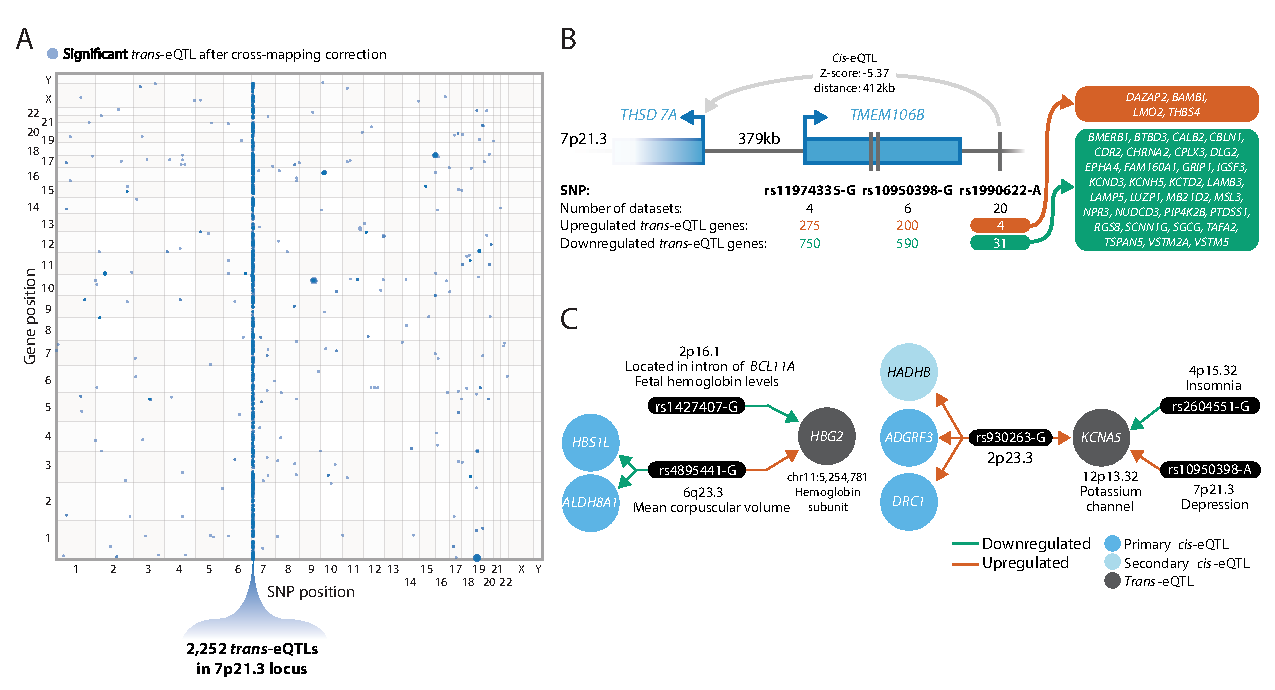
\includegraphics[width=\textwidth]{chapters/chapter5-brain-eqtls/img/2021-02-11-fig6-trans-eQTLs-v2.pdf}
	\caption{\textbf{\textit{Trans}-eQTLs in brain. (A)} Locus dot plot with the SNP position (x-axis) and gene position (y-axis) in the genome. Size of the dots is scaled by the p-value of the \textit{trans}-eQTL (larger is more significant). 7p21.3, the locus with most (83\%) of the \textit{trans}-eQTLs, is highlighted. (B) The three SNPs in the 7p21.3 locus and the number of datasets and number of up- and down-regulated \textit{trans}-eQTL genes each SNP has. For rs1990622, a frontotemporal lobar degenration SNP, the 35 genes it affects in \textit{trans}  and the 1 gene it affects in \textit{cis} are shown.  (C) Two examples of convergent effects from SNPs on genes. Left: \textit{trans}-eQTLs of rs1427407 and rs4895441 on HBG2 and right \textit{trans}-eQTL of rs930263, rs2604551, and rs10950398 on \textit{KCNA5}.}
	\label{metabrain_fig6}
\end{figure}

\Needspace{10\baselineskip}
\subsection{Brain co-regulation networks improve GWAS interpretation}
We generated brain-region specific co-regulation networks based on the RNA-seq data from the 8,544 samples (\textbf{Supplementary Note, Supplementary Figures 29-30}). We previously have done this for a heterogenous set of RNA-seq samples spanning across all available tissue types and cell lines (n=31,499)\cite{persBiologicalInterpretationGenomewide2015,deelenImprovingDiagnosticYield2019}, which showed that such a co-regulation network can be informative for interpreting GWAS studies\cite{persBiologicalInterpretationGenomewide2015} and helpful in the identification of new genes that cause rare diseases\cite{deelenImprovingDiagnosticYield2019}. 
	
We applied a new approach (‘\textit{Downstreamer}’ in preparation, see \textbf{Supplementary Note}) that improves upon DEPICT, our previously published post-GWAS pathway analysis method\cite{persBiologicalInterpretationGenomewide2015}. \textit{Downstreamer} can systematically determine which genes are preferentially co-regulated with genes that reside within GWAS loci. It does not use a significance threshold for a GWAS, but uses all SNP information. In addition, \textit{Downstreamer} accounts for LD and uses rigorous permutation testing to determine significance levels and control for Type I errors.

We applied \textit{Downstreamer} to schizophrenia (SCZ)\cite{ripkeBiologicalInsights1082014}, PD\cite{nallsIdentificationNovelRisk2019}, MS\cite{consortiumMultipleSclerosisGenomic2019}, AD\cite{kunkleGeneticMetaanalysisDiagnosed2019} and ALS GWAS summary statistics (\textbf{Supplementary Table 23-27}), using three different brain-derived co-regulation networks: one based on all 8,544 brain samples, one limited to 6,527 cortex samples and one limited to 715 cerebellum samples. We observed that there were multiple sets of genes that showed strong co-regulation with genes inside the GWAS loci for these diseases. For MS and AD, these were mostly immune genes, whereas for PD, ALS and SCZ these were genes that are specifically expressed in brain (\textbf{Supplementary Table 23-27}).  

For ALS, we applied \textit{Downstreamer} to summary statistics from a recent meta-analysis in individuals from European ancestry (\textbf{Supplementary Table 28}), and a trans-ethnic meta-analysis including European and Asian individuals (EUR+ASN; \textbf{Supplementary Table 23}; van Rheenen \textit{et al}., manuscript in preparation). To look for contributions of non-neurological cell types and tissues, we first used the previously published heterogenous network\cite{deelenImprovingDiagnosticYield2019} that comprises many different tissues and cell types, but did not identify genes that were significantly enriched for co-regulation with genes inside ALS loci. However, when we applied our method to the different brain co-regulation networks, we identified a set of 27 unique co-regulated genes (EUR+ASN summary statistics; \textbf{Figure \ref{metabrain_fig7}A; Supplementary Table 23}), depending on the type of brain co-regulation network used. \textit{HUWE1} was shared between the brain and cortex co-regulation network analysis, while \textit{UBR4} was shared between the cortex and cerebellum analysis. \textit{UBR4} is a ubiquitin ligase protein expressed throughout the body. A private \textit{UBR4} mutation, segregated with episodic ataxia in a large three-generation Irish family, implicates its role in muscle coordination\cite{conroyNovelLocusEpisodic2014}. \textit{UBR4} interacts with the $Ca^{2+}$ binding protein, calmodulin and $Ca^{2+}$ dysregulation has been linked to proteins encoded by ALS disease genes and motor neuron vulnerability\cite{lealCalciumDysregulationLinks2015}. We observed in the \textit{Downstreamer} findings that many of these prioritized genes are co-regulated with each other (\textbf{Figure \ref{metabrain_fig7}B}), and using our recently developed clinical symptom prediction algorithm\cite{deelenImprovingDiagnosticYield2019}, there was an enrichment of genes implicated in causing gait disturbances (\textbf{Figure \ref{metabrain_fig7}C}). These genes are associated with ALS (highlighted in blue), brain-related disorders (including \textit{DNAJC5}, \textit{HTT}, \textit{HUWE1}, \textit{TSC1} and \textit{YEATS2}) or muscle-related disorders (including \textit{KMT2B}). While various loci have been identified for both familial and sporadic forms of ALS, the function of the positional candidate genes within these loci is still unclear. Our Downstreamer analysis identified genes that show strong coregulation with positional candidate genes inside ALS loci, suggesting that these positional candidates must have a shared biological function. 

For MS, the heterogeneous network, including many blood and immune cell type samples, identified 257 unique genes that showed significantly enriched co-regulation with genes inside MS loci (\textbf{Figure \ref{metabrain_fig7}D; Supplementary Table 27}), and many were immune genes, which is also expected for this disease. However, when we applied the brain co-regulation networks, we identified a much smaller set of genes, and these genes showed strong enrichment for genes involved in the neurotrophin signaling pathway (\textbf{Figure \ref{metabrain_fig7}E and F}). Neurotrophins are polypeptides secreted by immunological cell types. In the brain, neurotrophin concentrations are important to promote the survival and proliferation of neurons as well as synaptic transmission. In MS patients, neurotrophin reactivity is higher in MS plaques, whereby neurotrophins are released by peripheral immune cells directly to the inflammatory lesions, suggesting a protective role of this signaling process\cite{kalinowskalyszczarzRoleNeurotrophinsMultiple2012,kerschensteinerActivatedHumanCells1999}. Neutrophins are also released by glial cells in the brain, including microglia and astrocytes, and their role in stimulating neuronal growth and survival could also contribute to an overall neuroprotective effect\cite{desantiNeuroinflammationNeuroprotectionUpdate2011}. In the heterogeneous network, we observed high expression for these genes in immune-related tissues (\textbf{Supplementary Figure 31A}), supporting the “outside-in hypothesis” that the immune system may be a potential trigger for MS\cite{consortiumMultipleSclerosisGenomic2019,baecherallanMultipleSclerosisMechanisms2018}. The brain specific network showed high expression in spinal cord and cerebellum but lower expression in cortex samples (\textbf{Supplementary Figure 31B}), which could be highlighting the specific biological processes taking place in these CNS regions that lead to disease. For example, the cerebellum is responsible for muscle coordination and ataxia occurs in approximately 80\% of MS patients with symptoms\cite{redondoPurkinjeCellPathology2015}. We speculate that both dysregulation of the immune system and dysregulation of certain neurological processes is a prerequisite for developing MS. 

\begin{figure}[H]
	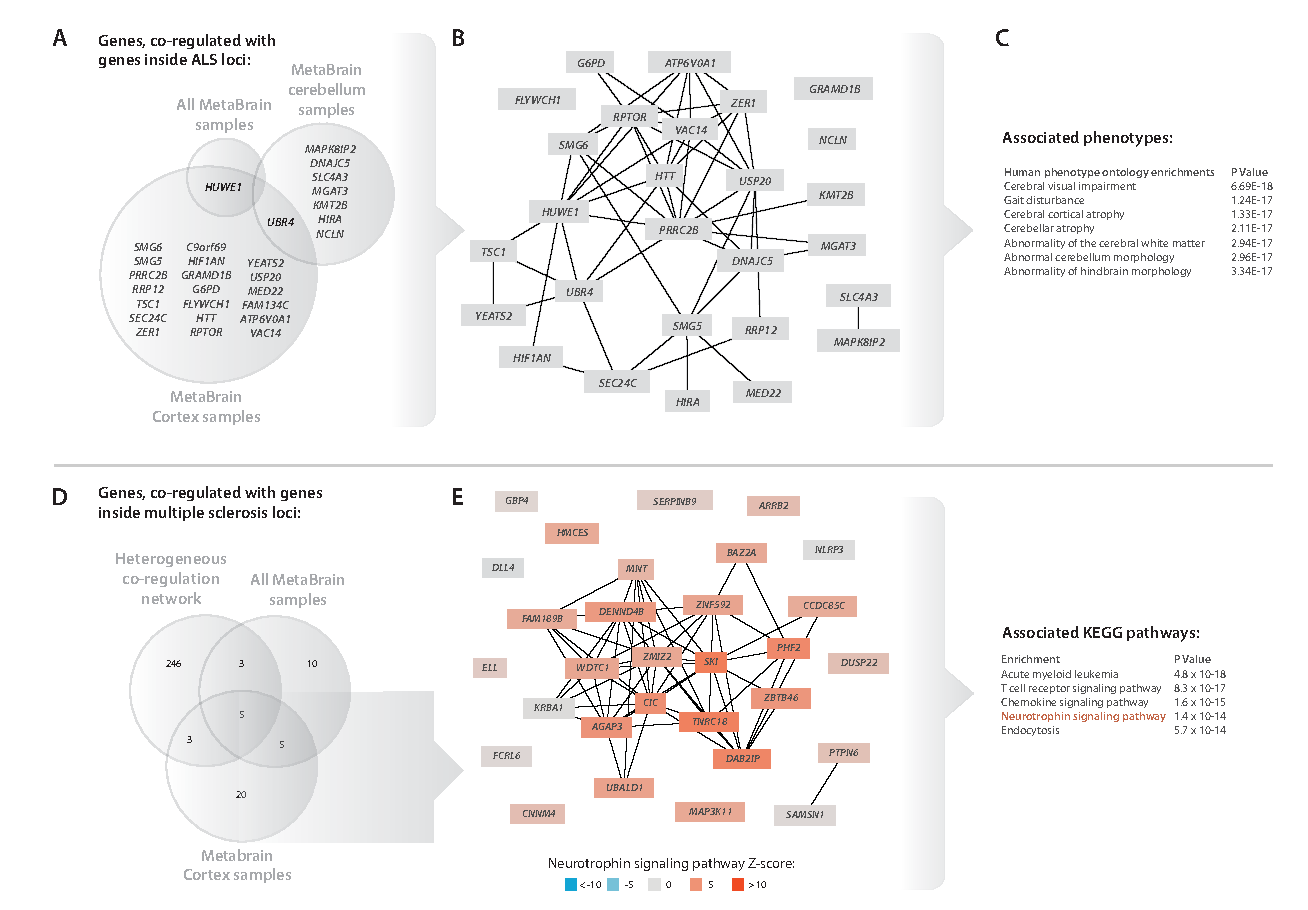
\includegraphics[width=\textwidth]{chapters/chapter5-brain-eqtls/img/2021-02-11-fig7-ALSPrioritizedCoreGenes-v2.pdf}
	\caption{\textbf{Gene co-regulation (A)} Genes that are co-regulated with genes that are within ALS loci. Co-regulation scores between genes are calculated using all \textit{MetaBrain} samples, only \textit{MetaBrain} cerebellum samples, or only \textit{MetaBrain} cortex samples. Except for \textit{URB4}, cortex and cerebellum networks find different co-regulated genes for ALS. (B) Co-regulation network using all \textit{MetaBrain} samples for all genes prioritized for ALS by \textit{Downstreamer}. (C) Top 7 Human Phenotype Ontology (HPO) enrichment for the \textit{Downstreamer} prioritzed ALS genes. (D) Genes that are co-regulated with genes that are within multiple sclerosis loci. Co-regulation scores between genes are calculated using a heterogeneous multi-tissue network, only \textit{MetaBrain} cerebellum samples, or only \textit{MetaBrain} cortex samples. Most genes are found using a large heterogenous co-regulation network. (E) Co-regulation network of all \textit{MetaBrain} samples for 33 genes prioritized by \textit{Downstreamer} in cortex. Genes are colored by their Z-scores of how well they fit within the neutrophin signaling pathway. (F) Top 5 KEGG enrichments for the \textit{Downstreamer }prioritized multiple sclerosis genes in cortex.}
	\label{metabrain_fig7}
\end{figure}

\Needspace{10\baselineskip}
\section{Discussion}

We here describe an integrated analysis of the effects of genetic variation on gene expression levels in brain in over 3,000 unique individuals. This sample size yielded sufficient statistical power to identify robust \textit{cis}-eQTL and to our knowledge for the first-time brain \textit{trans}-eQTLs that emanate from SNPs that have been previously linked to neurodegenerative or psychiatric phenotypes. 

We compared \textit{cis}-eQTLs in \textit{MetaBrain} to \textit{cis}-eQTLs in eQTLgen, a set of 31,684 blood samples. We observe a large proportion of shared \textit{cis}-eQTLs between brain and blood, most of which have the same allelic direction of effect. Our analysis also permitted us to identify \textit{cis}-eQTL effects that are independent of the primary \textit{cis}-eQTLs. Some of these independent effects reflect SNPs that are also the index variants for several neurological and psychiatric disorders, making them particularly interesting for subsequent follow-up. Recent observations have revealed that SNPs with the strongest \textit{cis}-eQTL effects are depleted for GWAS associations\cite{wangEnhancerDomainsPredict2020}. Thus, secondary, tertiary or quaternary \textit{cis}-eQTL SNPs could potentially be even more interesting to follow-up than certain primary \textit{cis}-eQTL SNPs to link association signals to function.

We studied different regions in the brain, permitting us to identify brain-region specific eQTLs. For this, to exclude spurious differences that may arise from different cell type proportions across brain regions, we first inferred cell type percentages for the major brain cell types. We then applied an eQTL interaction model (i.e., using the cell type percentage x genotype as interaction term), permitting us to identify 1,515 \textit{cis}-eQTLs that show cell type specificity. Most of these cell type dependent effects were observed for oligodendrocytes and neurons, the two most common cell types in the brain for which statistical power to observe such effects was the strongest. Still, we could identify 461 cell type dependent eQTLs also for macrophages, endothelial cells, or astrocytes. While we found strong concordance with immunohistochemistry results, our findings are largely based on a deconvolution approach, which in future studies will benefit from validation in purified cell types, e.g. using population-based single-cell RNA-seq datasets as they are now becoming available\cite{wijstSinglecellRNASequencing2018,PopulationscaleSinglecellRNAseq}. Such single-cell eQTL studies can gain substantial statistical power by limiting analyses to the large set of primary, secondary, tertiary and quaternary \textit{cis}-eQTLs our study reveals for bulk brain samples. 

To our knowledge, this is the best powered Mendelian randomization and colocalization analysis using brain \textit{cis}-eQTLs as instruments for bipolar disease, epilepsy, frontotemporal dementia, multiple sclerosis, cognitive function and years of schooling GWAS outcomes. Interestingly, also for schizophrenia three signals for \textit{CILP2}, \textit{MAU2} and \textit{TM6SF2} met our criteria that had not been reported in a recent psychiatric genomics consortium study\cite{consortiumMappingGenomicLoci2020}, further emphasizing the value of our well-harmonized, large eQTL data set in the tissue type of interest (\textbf{Supplementary Note}). Our results also identify increased \textit{CYP24A1} expression as associated with multiple sclerosis risk and propose neurons as the most susceptible cell type to \textit{CYP24A1} expression changes and likely active vitamin D levels. The potentially novel role of \textit{CYP24A1} in brain could play an important role in MS etiology, as may lowered expression of \textit{CLECL1} in microglia. 

The 2,589 identified \textit{trans}-eQTLs allowed us to gain insights into downstream molecular consequences of several disease-associated genetic variants. We observed that variants that are brain \textit{cis}-eQTLs more often show also \textit{trans}-eQTL effects than expected by chance, indicating functional consequences beyond the gene regulated in \textit{cis}. Our \textit{trans}-eQTL analysis focused on a single brain region and SNPs with a known interpretation (i.e. trait-associated variants and \textit{cis}-eQTL SNPs). We therefore expect that a genome-wide approach will identify many more \textit{trans}-eQTLs. 2,218 of the \textit{trans}-eQTLs were located in a 7p21.3 locus and the genes were strongly correlated with neuron proportions, indicating that cell type proportions can heavily impact \textit{trans}-eQTL identification. However, 21 of these \textit{trans}-eQTLs replicated in snRNA-seq data, suggesting that some of these \textit{trans}-eQTLs may also exist in single cells. Excluding the 7p21.3 locus, we identified 371 \textit{trans}-eQTLs located elsewhere in the genome, which are less likely due to neuron proportion differences. For several neurological and psychiatric conditions, our analyses indicate pathways that may help to elucidate disease causes and putative intervention points for future therapies.  

We used the brain-specific co-regulation networks to study several brain-related GWAS studies, with the aim to prioritize genes that show significantly enriched co-regulation with genes inside the associated GWAS loci. For ALS this revealed a limited, but significant set of genes which do not map within associated ALS loci, but that link genes within multiple ALS loci. Follow-up research on these prioritized genes might therefore help to better understand the poorly understood causal pathways that cause ALS. While it is tempting to speculate that these prioritized genes might represent genes that could serve as potential targets for pharmaceutical intervention, follow-up research is needed in order to establish whether these genes play a relevant role in ALS. 

Our study had several limitations. For instance, we performed single tissue eQTL analyses that were limited to a single RNA-seq sample per individual, excluding many RNA-seq samples from the analysis. A joint analysis across tissues, including multiple RNA-seq samples per individual using for example random effects models would further improve power\cite{davenportDiscoveringVivoCytokineeQTL2018,gtexconsortiumGeneticEffectsGene2017}, which would be especially useful for the future identification of \textit{trans}-eQTLs. Additionally, LD overlap analysis, Mendelian randomization and colocalization are sensitive to many factors, including eQTL and GWAS study sample size, effect size, variant density, LD structure and imputation quality. Differences between study designs may consequently influence the results of such analyses. For example, our colocalization and LD overlap analysis did not include the \textit{MAPT} gene for Alzheimer’s disease. The effect sizes of the \textit{cis}-eQTLs for this gene were limited in our study, since our alignment strategy could not account for the different long-range haplotypes in this locus causing the H1/H2 haplotype separating SNP rs8070723 to have a p-value of 0.2 (\textbf{Supplementary Note}). We note that this might be an issue for other genes as well. Future studies using graph-based alignment tools or long read sequencing methods would be required to ultimately determine the true effects on such genes. Our approach combined Mendelian randomization and colocalization, as it is possible for the \textit{cis}-eQTL instrument to coincidentally share association with the GWAS trait due to surrounding LD patterns in the genomic region. We opted to perform single SNP MR because other approaches, such as inverse variance weighted\cite{hemaniMRBasePlatformSupports2018} (IVW) MR, pool the estimates across many SNP instruments, which for many genes were not available. Potentially, methods such as IVW could be applied to our dataset in the future when genome-wide \textit{trans}-eQTL analysis would identify many more independent instruments per gene. However, MR analyses using QTLs could be susceptible to confounding because of horizontal pleiotropy\cite{hemaniEvaluatingPotentialRole2018}, where a single gene is affected by multiple indirect effects, which is likely to be exacerbated by including \textit{trans}-eQTLs. Our colocalization analysis used a more lenient posterior probability (PP4) threshold of $>$0.7, which we selected because we performed colocalization only in loci having a significant MR signal, limiting potential false positives. However, our colocalization approach assumed the presence of a single association in each locus, which might not be optimal for \textit{cis}-eQTL loci harboring multiple independent variants, such as for the \textit{TREM2} gene (\textbf{Supplementary Note}). Consequently, our approach may have not detected colocalizing signals in some loci. Recently, colocalization methods were published\cite{wallaceElicitingPriorsRelaxing2020} that do not have this assumption, and consequently may improve future colocalization results.      

With the numbers of GWAS loci for brain-related traits and diseases steadily climbing, we expect that our resource will prove itself as a highly valuable toolkit for post-GWAS brain research and beyond. Among others, we demonstrate how our dataset can be utilized to disambiguate GWAS loci, point to causal pathways and prioritize targets for drug discovery. To our knowledge, this is the largest non-blood eQTL analysis ever conducted, providing insights into the functional consequences of many disease associated variants. We expect that through future integration with single-cell eQTL studies that have higher resolution but lower power, our results will help to pinpoint transcriptional effects in specific brain cell types for many disease-associated genetic variants. 

\Needspace{10\baselineskip}
\section{Material \& Methods}
\Needspace{10\baselineskip}
\subsection{Dataset collection and description }
We collected human brain bulk RNA-seq datasets from different resources. Briefly, we collected previously published samples from the AMP-AD consortium (AMP-AD MAYO\cite{hodesAcceleratingMedicinesPartnership2016}, ROSMAP\cite{hodesAcceleratingMedicinesPartnership2016} and MSBB\cite{hodesAcceleratingMedicinesPartnership2016}) and the PsychENCODE consortium (Bipseq\cite{wangComprehensiveFunctionalGenomic2018}, BrainGVEX\cite{wangComprehensiveFunctionalGenomic2018}, CMC\cite{fromerGeneExpressionElucidates2016}, GVEX, LIBD, and UCLA\_ASD\cite{wangComprehensiveFunctionalGenomic2018}) from Synapse.org using the Python package synapseclient\cite{teamSynapseclientClientSynapse}. The NABEC and GTEx datasets were retrieved from NCBI dbGaP, and TargetALS was provided directly by the investigators. For an overview of the number of samples per dataset, see \textbf{Supplementary Table 1}. 

Additionally, we collected public brain bulk RNA-seq samples from the European Nucleotide Archive (ENA; \textbf{Supplementary Table 28}). To select only the brain samples, we first downloaded the SkyMap database\cite{tsuiExtractingAllelicRead2018}, which provides readily mapped read counts and sample annotations. We performed rigorous quality control on this dataset, and selected ENA, excluding for example brain cell lines, brain cancer samples, and samples with RNA spike ins (See \textbf{Supplementary Note} for more details on this method, \textbf{Supplementary Figure 1}), resulting in 1,759 samples, and 9,363 samples when combined with the previously published datasets \textbf{Supplementary Table 1}. 

\Needspace{10\baselineskip}
\subsection{RNA-seq data}
RNAseq data was processed using a pipeline built with molgenis-compute\cite{byelasMOLGENISBasedComputational2011}. FastQ files were aligned against the GENCODE\cite{frankishGENCODEReferenceAnnotation2019} v32 primary assembly with STAR\cite{dobinSTARUltrafastUniversal2013} (version 2.6.1c), while excluding patch sequences (see \textbf{Supplementary Note}) with parameter settings: outFilterMultimapNmax = 1, twopassMode Basic, and outFilterMismatchNmax = 8 for paired-end sequences, outFilterMismatchNmax = 4 for single-end sequences. Gene quantification was performed by STAR, similar to gene quantification using HTSeq\cite{andersHTSeqPythonFramework2015} with default settings. The gene counts were then TMM\cite{robinsonScalingNormalizationMethod2010} normalized per cohort using edgeR\cite{robinsonEdgeRBioconductorPackage2010} (version 3.20.9) with R\cite{rcoreteamLanguageEnvironmentStatistical2017} (version 3.5.1). 

To measure FastQ and alignment quality we used FastQC\cite{BabrahamBioinformaticsFastQC} version 0.11.3), STAR\cite{dobinSTARUltrafastUniversal2013} metrics, and Picard Tools\cite{broadinstitutePicardTools2019} (version 2.18.26) metrics (MultipleMetrics, and RNAseqMetrics). Samples were filtered out if aligned reads had $<$ 10
\% coding bases (\textbf{Supplemental Figure 3B}), $<$ 60\% reads aligned (\textbf{Supplemental Figure 3B}), or $<$ 60\% unique mapping. 117 of the RNA-seq samples did not pass this filter, mostly from GTEx\cite{consortiumGTExConsortiumAtlas2020}. The other quality measurements were visually inspected but contained no outliers. 

RNA-sequencing library preparation, and other technical factors can greatly influence the ability to quantify of gene expression. Therefore, for a given sample such factors often influence the total variation. For example, such issues can be caused by problems during RNA-seq library preparation that lead to an increased number of available transcripts to quantify, or conversely, a lack of variation in quantified transcripts (compared to other samples in the dataset). We therefore opted to identify RNA-seq outliers that were not explained by poor RNA-seq alignment metrics. For this purpose, we performed PCA on the RNA data prior to normalization: we reasoned that the first two components capture excess or depletion of variation caused by technical problems. We identified 20 RNA-seq outliers with PC1 score $>$4 standard deviation away from the mean (\textbf{Supplementary Figure 3A}). Twenty outlier samples were removed and the principal components were recalculated  (\textbf{Supplementary Figure 3B}). We detected and removed 45 additional outlier samples. We confirmed no additional outlier samples in the third iteration and principal component calculation (\textbf{Supplementary Figure 3C}), and 8,868 samples were taken through additional QC. 

We next removed genes with no variation and then log2-transformated, quantile normalized, and Z-score transformed the RNA-seq counts per sample. PCA on the normalized expression data showed that datasets strongly cluster together (\textbf{Supplementary Figure 4A}), likely due to dataset specific technical differences (e.g. single-end versus paired-end sequencing). To correct for this the normalized expression data was correlated against 77 covariates from different QC tools (FastQC\cite{BabrahamBioinformaticsFastQC}, STAR\cite{dobinSTARUltrafastUniversal2013}, and Picard Tools\cite{broadinstitutePicardTools2019}), such as percent protein coding, GC content, and 5’ prime/3’ prime bias. The top 20 correlated technical covariates (\% coding bases, \% mRNA bases, \% intronic bases, median 3’ prime bias, \% usable bases, \% intergenic bases, \% UTR bases, \% reads aligned in pairs, average mapped read length, average input read length, number of uniquely mapped reads, \% reads with improper pairs, number of reads improper pairs, total sequences, total reads, \% chimeras, number of HQ aligned reads, number of reads aligned, HQ aligned Q20 bases, HQ aliged bases) were regressed out of the expression data using a linear model. After covariate correction, clustering of datasets in PC 1 and PC 2 was no longer present (\textbf{Supplementary Figure 4B}).  

Our collection of RNA-seq samples consisted of 36 different tissue labels, many of which were represented by only a few samples. Therefore, we next defined major brain regions present in our dataset, including samples from amygdala, basal ganglia, cerebellum, cortex, hippocampus and spinal cord. We noted that some samples (especially from ENA) were not annotated with a specific major brain region. To resolve this, we performed PCA over the sample correlation matrix and then performed k-nearest neighbors on the first two PCs (k=7) to classify samples to the major brain regions. Using this approach, we defined a set of 86 amygdala, 574 basal ganglia, 723 cerebellum, 6,601 cortex, 206 hippocampus, 252 hypothalamus and 285 spinal cord samples (\textbf{Supplementary Table 1, Figure \ref{metabrain_fig2}A}). 

\Needspace{10\baselineskip}
\subsection{Genotype data and definition of eQTL datasets}
The genotype data for the included datasets was generated using different platforms, including genotypes called from whole genome sequencing (WGS; AMP-AD, TargetALS\cite{prudencioDistinctBrainTranscriptome2015}, GTEx\cite{consortiumGTExConsortiumAtlas2020}), genotyping arrays (NABEC\cite{gibbsAbundantQuantitativeTrait2010}, Braineac\cite{ramasamyGeneticVariabilityRegulation2014}), and haplotype reference consortium (HRC)\cite{mccarthyReferencePanel642016} imputed genotypes (PsychENCODE datasets), or were called from RNA-seq directly (ENA dataset; see \textbf{Supplementary Note}). In total, 22 different genotyping datasets were available, reflecting 6,658 genotype samples (\textbf{Supplementary Table 1}).  

We performed quality control on each dataset separately, using slightly different approaches per platform. For the array-based datasets, we first matched genotypes using GenotypeHarmonizer\cite{deelenGenotypeHarmonizerAutomatic2014} using 1000 genomes phase 3 v5a (1kgp) as a reference, limited to variants having MAF $>$ 1\%, $<$ 95\% missingness and Hardy-Weinberg equilibrium p-value $<$ 0.0001. Genotypes were then imputed using HRC v1.1 as a reference on the Michigan imputation server 30. In all HRC imputed datasets, variants with imputation info score $<$ 0.3 were removed. For the WGS datasets, we removed indels and poorly genotyped SNPs having VQSR tranche $<$ 99.0, genotype quality $<$ 20, inbreeding coefficient $<$ -0.3 and $>$ 5\% missingness, setting genotype calls with allelic depth $<$ 10 and allelic balance $<$ 0.2 or $>$ 0.8 as missing. WGS datasets were not imputed with HRC. Considering the small size of some of the datasets, we decided to focus further analysis on variants with MAF $>$ 1\% and Hardy-Weinberg p-value $>$ 0.0001. 

In each dataset, we removed genetically similar individuals by removing individuals with pihat $>$ 0.125, as calculated with Plink. Additionally, we merged genotypes with those from 1kgp, pruned genotypes with -indep-pairwise 50 5 0.2 in plink, and performed PCA on the sample correlation matrix. We performed k-nearest neighbors (k=7) on the first two PCs, using the known ancestry labels in 1kgp, to assign an ancestry to each genotyped sample. The majority of included samples was of EUR descent: 5,138 samples had an EUR assignment, 805 samples had an AFR assignment, and 573 samples were assigned to the other ethnicities (\textbf{Supplementary Table 1}, \textbf{Figure \ref{metabrain_fig2}B}). 

For the purpose of eQTL analysis, we next assessed links between RNA-seq and genotype samples and noted that some individuals had multiple RNA-seq samples (e.g. from multiple brain regions) or multiple genotype samples (e.g. from different genotyping platforms). In total, we were able to determine 7,644 links between RNA-seq samples and genotype samples (Supplementary Table 1), reflecting 3,525 unique EUR individuals, 624 unique AFR individuals, and 510 unique individuals assigned to other ethnicities. We then grouped linked RNA-seq samples based on ethnicity and tissue group to prevent possible biases on eQTL results. For those individuals with multiple linked RNA-seq samples, we selected a sample at random within these groups. Within each tissue and ethnicity group, we then selected unique genotype samples across datasets in such a way to maximize sample size per genotype dataset. For the eQTL analysis per tissue, we only considered those datasets having more than 30 unique linked samples available, and for which at least two independent datasets were available. Using these criteria for sample and dataset selection, we were able to create 7 eQTL discovery datasets: Basal ganglia-EUR (n=208), Cerebellum-EUR (n=492), Cortex-EUR (n=2,970), Cortex-AFR (n=420), Hippocampus-EUR (n=168) and Spinal cord-EUR (n=108; \textbf{Supplementary Table 1, Figure \ref{metabrain_fig2}C}). 


\Needspace{10\baselineskip}
\subsection{eQTL analysis}
Our dataset consists of different tissues and ethnicities, and samples have been collected in different institutes using different protocols. Consequently, combining these datasets to perform eQTL analysis is complicated, due to possible biases each of these factors may introduce. To resolve this issue, we opted to perform an eQTL meta-analysis within each of the defined eQTL discovery datasets. To reduce the effect of possible gene expression outliers, we calculated Spearman’s rank correlation coefficients for each eQTL in each dataset separately, and then meta-analyzed the resulting coefficients using a sample size weighted Z-score method, as described previously\cite{vosaUnravelingPolygenicArchitecture2018}. While we acknowledge that this method may provide less statistical power than the commonly used linear regression, we chose this method to provide conservative effect estimates. To identify \textit{cis}-eQTLs, we tested SNPs located within 1 megabases (Mb) of the \textit{trans}cription start site, while for the identification of \textit{trans}-eQTLs, we required this distance to be at least 5mb. For both analyses, we selected variants having a MAF$>$1\%, and a Hardy-Weinberg p-value $>$ 0.0001. Using the GENCODE v32 annotation, we were able to quantify 58,243 genes, of which 19,373 are protein coding. While non-coding genes have been implicated to be important for brain function76, these genes generally have poor genomic and functional annotations, meaning that it is often unknown in which pathway they function, and that there is uncertainty about their genomic sequence. We therefore focused our eQTL analyses on protein coding genes. 

To correct for multiple testing, we reperformed the \textit{cis}- and \textit{trans}-eQTL analyses, while permuting the sample labels 10 times. Using the permuted p-values, we created empirical null distributions and determined a false discovery rate (FDR) as the proportion of unpermuted observations over the permuted observations and considered associations with FDR$<$0.05 as significant. To provide a more stringent FDR estimate for our \textit{cis}-eQTL results, we limited FDR estimation to the top associations per gene, as described previously\cite{vosaUnravelingPolygenicArchitecture2018}. We note that our FDR estimate is evaluated on a genome-wide level, rather than per gene, and consequently FDR estimates stabilize after a few permutations\cite{westraSystematicIdentificationTranseQTLs2013}. 

Since \textit{cis}-eQTL loci are known to often harbor multiple independent associations, we performed an iterative conditional analysis, where for each iteration, we regressed the top association per gene from the previous associations, and re-performed the \textit{cis}-eQTL analysis until no additional associations at FDR$<$0.05 could be identified. 

Since a genome-wide \textit{trans}-eQTL analysis would result in a large multiple testing burden considering the billions of potential tests, we limited this analysis to a set of 140,000 variants we considered to have a high probability of being \textit{trans}-eQTLs. This set constituted of variants that were either previously associated with traits, having a GWAS p-value $<$ 5x10-8 in available the IEU GWAS database\cite{lyonVariantCallFormat2020} and EBI GWAS catalog\cite{bunielloNHGRIEBIGWASCatalog2019} on May $3^{rd}$, 2020), and additional neurological traits (see \textbf{Supplemental Table 17}) or were showing an association with FDR$<$0.05 in any of our discovery \textit{cis}-eQTL analyses (including secondary, tertiary and quandary associations identified in the iterative conditional analysis).  \textit{Cis}-eQTLs in Cortex-EUR were highly concordant when replicated in Cortex-AFR (\textbf{Figure \ref{metabrain_fig3}C}). Consequently, to maximize the sample size and statistical power, we meta-analyzed Cortex-EUR and Cortex-AFR datasets together. However, for the \textit{trans}-eQTL analysis we omitted ENA, to prevent bias by genotypes called from RNA-seq samples. Additionally, For the \textit{trans}-eQTL analysis, we did not correct the gene expression data for 10 PCs, since \textit{trans}-eQTLs can be driven by cell proportion differences\cite{vosaUnravelingPolygenicArchitecture2018}, and many of the first 10 PCs in the \textit{MetaBrain}  dataset were correlated with estimated cell type proportions (\textbf{Supplementary Figure 32}). To test for \textit{trans}-eQTLs, we assessed those combinations of SNPs and genes where the SNP-TSS distance was $>$5 Mb, or where gene and SNP were on different chromosomes. We note that we did not evaluate eQTLs where the SNP-TSS distance was $>$1 Mb and $<$5 Mb, which potentially excludes detection of long-range \textit{cis}-eQTLs or short-range \textit{trans}-eQTLs. We expect however, that this excludes only a limited number of eQTLs, since we observed that this distance was $<$31Kb for 50\% of \textit{cis}-eQTLs (\textbf{Figure \ref{metabrain_fig3}B)}, indicating most \textit{cis}-eQTLs are short-ranged. Additionally, we reasoned that the $>$5 Mb cutoff would prevent identification of false-positive \textit{trans}-eQTLs due to long-range LD.  

\Needspace{10\baselineskip}
\subsection{Estimation of cell count proportions using non-negative least squares}
By leveraging the cell type specific gene expression collected through scRNA-seq, a bulk tissue sample can be modelled as a parts-based representation of the distinct cell types it consists of. In such a model, the weights of each part (i.e. cell type proportions) can be determined by deconvolution. In the deconvolution of the \textit{MetaBrain} bulk expression data we used a single-cell derived signature matrix including the five major cell types in the brain: neurons, oligodendrocytes, macrophages, endothelial cells and astrocytes. This signature matrix was generated in the context of the CellMap project (Zhengyu Ouyang \textit{et al}.; manuscript in preparation). In short, we created pseudo-bulk expression profiles by extracting gene expression values for specific cell types of interest from annotated single cell and single nuclei expression matrices. Using differential expression analysis and applying several rounds of training and testing, we selected 1,166 differentially expressed genes and calculated the average read counts per cell type. We then filtered out genes that had no variation in expression, leaving a total of 1,132 genes. We extracted the corresponding TMM normalized gene counts of these signature genes for all European cortex samples in \textit{MetaBrain}. After correcting the counts for cohort effects using OLS, but not for any other technical covariates, we applied log2 transformation on both the signature matrix as well as the bulk gene count matrix. Subsequently we applied non-negative least squares (NNLS)\cite{lawsonSolvingLeastSquares1995} using SciPy (version 1.4.1)\cite{virtanenSciPyFundamentalAlgorithms2020} to model the bulk expression as a parts-based representation of the single-nucleus derived signature matrix. First introduced by Lawson and Hanson\cite{lawsonSolvingLeastSquares1995}, NNLS method is the basis of numerous deconvolution methods to date. In short, NNLS attempt to find a non-negative weight (coefficient) for each of the cell types that, when summed together, minimizes the least-squares distance to the observed gene counts. Lastly, we transformed the resulting coefficients into cell type proportions by dividing them over the sum of coefficients for each sample. The resulting cell proportions are then used to identify cell type mediated eQTL effects. For this we applied Decon-eQTL\cite{raulaguirregamboaDeconvolutionBulkBlood2020} (version 1.4; default parameters) in order to systematically test for significant interaction between each cell type fractions and genotype, while also controlling for the effect on expression of the other cell types. The resulting p-values are then correct for multiple testing using the Benjamini-Hochberg method on a per-cell-type basis. 

\Needspace{10\baselineskip}
\subsection{Cell type specific ROSMAP single-nucleus datasets }

In order further confirm cell type specific eQTL effects, we used the ROSMAP single-nucleus data, encompassing 80,660 single-nucleus transcriptomes from the prefrontal cortex of 48 individuals with varying degrees of Alzheimer’s disease pathology\cite{mathysSinglecellTranscriptomicAnalysis2019}. We used Seurat version 3.2.2\cite{stuartComprehensiveIntegrationSingleCell2019} to analyze the data. First, we removed the genes that did not pass filtering as described previously\cite{mathysSinglecellTranscriptomicAnalysis2019}, leaving us with 16,866 genes and 70,634 cells for further analysis. After this, we normalized the expression matrix on a per individual per cell type basis using sctransform\cite{hafemeisterNormalizationVarianceStabilization2019} and visualized the normalized expression matrix using UMAP dimensionality reduction\cite{mcinnesUMAPUniformManifold2020}. We observed that cell types, as defined by Mathys \textit{et al}\cite{mathysSinglecellTranscriptomicAnalysis2019}., for the majority cluster together (\textbf{Supplementary Figures 33 and 34}). We then created expression matrices for each broad cell type (excitatory neurons, oligodendrocytes, inhibitory neurons, astrocytes, oligodendrocyte precursor cells, microglia, pericytes and endothelial cells) by calculating the average expression per gene and per individual basis. We then used these cell-type datasets for eQTL mapping using the same procedure as the bulk data. To correct for multiple testing, we confined the analysis to only test for primary \textit{cis}- and \textit{trans}-eQTLs found in \textit{MetaBrain}  cortex, while also permuting the sample labels 100 times. Lastly, we calculated the Spearman correlation between gene expression levels and genotypes and their 95\% confidence intervals\cite{bonettSampleSizeRequirements2000}.  

\Needspace{10\baselineskip}
\subsection{Single SNP Mendelian Randomization analysis}
Mendelian Randomization (MR) was conducted between the Cortex-EUR \textit{MetaBrain}  eQTLs and 23 neurological/psychiatric traits and 8 brain volume traits from ENIGMA (\textbf{Supplementary Table 11}). Cortex-EUR eQTLs at genome-wide significant (P $< 5 \times 10^{-08}$) were selected and then LD clumped to obtain independent SNPs to form our set of instruments. LD clumping was carried out using the ld\_clump() function in the ieugwasr package (\url{https://mrcieu.github.io/ieugwasr/}) on the default settings (10,000 kb clumping window with r2 cut-off of 0.001 using the 1000 Genomes EUR reference panel). SNP associations for each of the eQTL instruments were then looked up in the outcome GWASs of interest. If the SNP could not be found in the outcome GWAS using a direct lookup of the dbSNP rsid, then a proxy search was performed to extract the next closest SNP available in terms of pairwise LD, providing minimum r2 threshold of 0.8 with the instrument. Outcome GWAS lookup and proxy search was performed using the associations() function in the ieugwasr package. To ensure correct orientation of effect alleles between the eQTL instrument and outcome GWAS associations, the SNP effects were harmonized using the harmonise\_data() in TwoSampleMR (\url{https://mrcieu.github.io/TwoSampleMR/}). Action 2 was selected which assumes that the alleles are forwarded stranded in the GWASs (i.e. no filtering or re-orientation of alleles according to frequency was conducted on the palindromic SNPs). Single SNP MR was then performed on the harmonized SNP summary statistics using the mr\_singlesnp() function in TwoSampleMR. Single SNP MR step computes a Wald ratio, which estimates the per unit change in gene expression per change in risk for the outcome, explained through the effect allele of the instrumenting SNP. We reported all the MR findings that passed the suggestive threshold of $5 \times 10^{-05}$. The threshold of significance adjusting for multiple testing correction is $p=1.865 \times 10^{-7}$. We did not implement multi-SNP analysis (such as the Inverse Variance Weighted method), because there are a small number of instrumenting SNPs available per gene, which would result in unreliable MR estimates for most of the genes. 

\Needspace{10\baselineskip}
\subsection{Colocalization}
Following the MR analysis, colocalization analysis was performed on the MR findings that passed the suggestive threshold to determine if the eQTL and trait shared the same underlying signal. We run colocalization using both the default parameters (p1=p2=10-4 and p12=10-5) and parameters based on the number of SNPs in the region (p1=p2=1/(number of SNPs in the region) and p12 = p1 /10). We consider the two traits, eQTL and GWAS outcome, passes colocalization if either of the two parameters yields PP4 $>$0.7. Additionally, colocalization was systematically analyzed against one trait to compare to robustness of the Cortex-EUR eQTLs with existing cortex eQTL data sets (see \textbf{Supplementary Note}). 

\Needspace{10\baselineskip}
\section*{URLs}
\textbf{Picard}: \url{http://broadinstitute.github.io/picard/} \\
\textbf{dbGAP}: \url{https://dbgap.ncbi.nlm.nih.gov/} \\
\textbf{European Nucleotide Archive}: \url{http://www.ebi.ac.uk/ena} \\
\textbf{Metabrain}: \url{https://metabrain.nl } \\
\textbf{ieugwasr package}: \url{https://mrcieu.github.io/ieugwasr/} \\
\textbf{TwoSampleMR}: \url{https://mrcieu.github.io/TwoSampleMR/ }

\Needspace{10\baselineskip}
\section*{Accessions}
\textbf{TargetALS} TargetALS data was pushed directly from the NY Genome center to our sftp server. \\
\textbf{CMC} CMC data was downloaded from \url{https://www.synapse.org/}. Accession code: syn2759792 \\
\textbf{GTEx} GTEx was downloaded from SRA using fastq-dump of the SRA toolkit. Access has been requested and granted through dbGaP. \\
\textbf{Braineac} Braineac data has been pushed to our ftp server by Biogen. 
\textbf{AMP-AD} AMP-AD data has been downloaded from synapse. Accession code: syn2580853 
\textbf{ENA} ENA data has been downloaded from the European Nucleotide Archive.
\textbf{CMC\_HBCC} CMC\_HBCC data was downloaded from \url{https://www.synapse.org/}. Accession code: syn10623034 \\
\textbf{BrainSeq} BrainSeq data was downloaded from \url{https://www.synapse.org/}. Accession code: syn12299750 \\
\textbf{UCLA\_ASD} UCLA\_ASD data was downloaded from \url{https://www.synapse.org/}. Accession code: syn4587609 \\
\textbf{BrainGVEx} BrainGVEx data was downloaded from \url{https://www.synapse.org/}. Accession code: syn4590909 \\
\textbf{BipSeq} BipSeq data was downloaded \url{from https://www.synapse.org/}. Accession code: syn5844980 \\
\textbf{GTEx} GTEx data was downloaded from dbgap. \\
Accession code: phs000424.v7.p2 \\
\textbf{NABEC} NABEC data was downloaded from dbgap. \\
Accession code: phs001301.v1.p1 \\
\textbf{CellMap} single-cell and single-nuclei RNA-seq datasets were downloaded from Gene Expression Omnibus (GEO), BioProject, the European Genome-phenome Archive (EGA) and the Allan Brain Atlas. \\
Accession codes: GSE97930, GSE126836, GSE103723, GSE104276, PRJNA544731, PRJNA434002, phs000424, phs001836. 

\Needspace{10\baselineskip}
\section*{Acknowledgements}
We thank the donors of the brain tissues underlying the RNA-seq data used for this study and their families for their willingness to donate samples for research. We would like to thank the Center for Information Technology of the University of Groningen for their support and for providing access to the Peregrine high-performance computing cluster, as well as the UMCG Genomics Coordination center, the UG Center for Information Technology and their sponsors BBMRI-NL and TarGet for storage and compute infrastructure. We would like to greatly thank all researchers involved with the following projects for making their data available for use. E.A.T., Y.H., C.-Y.C, E.E.M., M.I.Z. and H.R. are employed by Biogen. D.B. and T.R.G. are supported by funding from the UK Medical Research Council (MRC Integrative Epidemiology Unit at the University of Bristol, MC\_UU\_00011/4) and a sponsored research collaboration with Biogen. L.F. is supported by grants from the Dutch Research Council (ZonMW-VIDI 917.14.374 to L.F.), by an ERC Starting Grant, grant agreement 637640 (ImmRisk), by an Oncode Senior Investigator grant and a sponsored research collaboration with Biogen. This project has received funding from the European Research Council (ERC) under the European Union's Horizon 2020 research and innovation programme (grant agreement n 772376 - EScORIAL. The authors thank the Biogen CellMap team (Z. Ouyang, N. Bourgeois, E. Lyashenko, P. Cundiff, K. Li, X. Zhang, F. Casey, S. Engle, R. Kleiman, B. Zhang and M. Zavodszky) for the expertise and advice provided toward deriving the cell-type specific expression profiles. 

\Needspace{10\baselineskip}
\subsection*{ROSMAP}

The results published here are in whole or in part based on data obtained from the AMP-AD Knowledge Portal (doi:10.7303/syn2580853). Study data were provided by the Rush Alzheimer’s Disease Center, Rush University Medical Center, Chicago. Data collection was supported through funding by NIA grants P30AG10161, R01AG15819, R01AG17917, R01AG30146, R01AG36836, U01AG32984, U01AG46152, the Illinois Department of Public Health, and the \textit{trans}lational Genomics Research Institute. 
Genotype data: \url{doi:10.1038/mp.2017.20}. RNAseq: \url{doi:10.1038/s41593-018-0154-9}.  

\Needspace{10\baselineskip}
\subsection*{Mayo}

The results published here are in whole or in part based on data obtained from the AMP-AD Knowledge Portal (doi:10.7303/syn2580853). Study data were provided by the following sources: The Mayo Clinic Alzheimer’s Disease Genetic Studies, led by Dr. Nilufer Taner and Dr. Steven G. Younkin, Mayo Clinic, Jacksonville, FL using samples from the Mayo Clinic Study of Aging, the Mayo Clinic Alzheimer’s Disease Research Center, and the Mayo Clinic Brain Bank. Data collection was supported through funding by NIA grants P50 AG016574, R01 AG032990, U01 AG046139, R01 AG018023, U01 AG006576, U01 AG006786, R01 AG025711, R01 AG017216, R01 AG003949, NINDS grant R01 NS080820, CurePSP Foundation, and support from Mayo Foundation. Study data includes samples collected through the Sun Health Research Institute Brain and Body Donation Program of Sun City, Arizona. The Brain and Body Donation Program is supported by the National Institute of Neurological Disorders and Stroke (U24 NS072026 National Brain and Tissue Resource for Parkinsons Disease and Related Disorders), the National Institute on Aging (P30 AG19610 Arizona Alzheimer’s Disease Core Center), the Arizona Department of Health Services (contract 211002, Arizona Alzheimer’s Research Center), the Arizona Biomedical Research Commission (contracts 4001, 0011, 05-901 and 1001 to the Arizona Parkinson's Disease Consortium) and the Michael J. Fox Foundation for Parkinson’s Research.  doi:10.1038/sdata.2016.89 


\Needspace{10\baselineskip}
\subsection*{MSBB}
The results published here are in whole or in part based on data obtained from the AMP-AD Knowledge Portal (doi:10.7303/syn2580853). These data were generated from postmortem brain tissue collected through the Mount Sinai VA Medical Center Brain Bank and were provided by Dr. Eric Schadt from Mount Sinai School of Medicine. 

\Needspace{10\baselineskip}
\subsection*{CMC}

Data were generated as part of the CommonMind Consortium supported by funding from Takeda Pharmaceuticals Company Limited, F. Hoffman-La Roche Ltd and NIH grants R01MH085542, R01MH093725, P50MH066392, P50MH080405, R01MH097276, RO1-MH-075916, P50M096891, P50MH084053S1, R37MH057881, AG02219, AG05138, MH06692, R01MH110921, R01MH109677, R01MH109897, U01MH103392, and contract HHSN271201300031C through IRP NIMH. Brain tissue for the study was obtained from the following brain bank collections: the Mount Sinai NIH Brain and Tissue Repository, the University of Pennsylvania Alzheimer’s Disease Core Center, the University of Pittsburgh NeuroBioBank and Brain and Tissue Repositories, and the NIMH Human Brain Collection Core. CMC Leadership: Panos Roussos, Joseph Buxbaum, Andrew Chess, Schahram Akbarian, Vahram Haroutunian (Icahn School of Medicine at Mount Sinai), Bernie Devlin, David Lewis (University of Pittsburgh), Raquel Gur, Chang-Gyu Hahn (University of Pennsylvania), Enrico Domenici (University of Trento), Mette A. Peters, Solveig Sieberts (Sage Bionetworks), Thomas Lehner, Stefano Marenco, Barbara K. Lipska (NIMH). 

\Needspace{10\baselineskip}
\subsection*{GTEx}

The Genotype-Tissue Expression (GTEx) Project was supported by the Common Fund of the Office of the Director of the National Institutes of Health (commonfund.nih.gov/GTEx). Additional funds were provided by the NCI, NHGRI, NHLBI, NIDA, NIMH, and NINDS. Donors were enrolled at Biospecimen Source Sites funded by NCI\\Leidos Biomedical Research, Inc. subcontracts to the National Disease Research Interchange (10XS170), Roswell Park Cancer Institute (10XS171), and Science Care, Inc. (X10S172). The Laboratory, Data Analysis, and Coordinating Center (LDACC) was funded through a contract (HHSN268201000029C) to the The Broad Institute, Inc. Biorepository operations were funded through a Leidos Biomedical Research, Inc. subcontract to Van Andel Research Institute (10ST1035). Additional data repository and project management were provided by Leidos Biomedical Research, Inc.(HHSN261200800001E). The Brain Bank was supported supplements to University of Miami grant DA006227. Statistical Methods development grants were made to the University of Geneva (MH090941 \& MH101814), the University of Chicago (MH090951, MH090937, MH101825, \& MH101820), the University of North Carolina - Chapel Hill (MH090936), North Carolina State University (MH101819), Harvard University (MH090948), Stanford University (MH101782), Washington University (MH101810), and to the University of Pennsylvania (MH101822). The datasets used for the analyses described in this manuscript were obtained from dbGaP at \url{http://www.ncbi.nlm.nih.gov/gap} through dbGaP accession number phs000424.v7.p2 on 02/27/2020. 

\Needspace{10\baselineskip}
\subsection*{NABEC}
Data was collected from dbGAP accession phs001301.v1.p1, which was generated by J. R. Gibbs, M. van der Brug, D. Hernandez, B. Traynor, M. Nalls, S-L. Lai, S. Arepalli, A. Dillman, I. Rafferty, J. Troncoso, R. Johnson, H. R. Zielke, L. Ferrucci, D. Longo, M.R. Cookson, and A.B. Singleton. The NABEC dataset was generated at National Institute on Aging, Bethesda, MD, USA, Institute of Neurology, University College London, London, UK, The Scripps Research Institute, Jupiter, FL, USA, Johns Hopkins University, Baltimore, MD, USA, and the University of Maryland Medical School, Baltimore, MD, USA. NABEC was funded by Z01 AG000949-02. National Institutes of Health, Bethesda, MD, USA and Z01 AG000015-49. National Institutes of Health, Bethesda, MD, USA. 

\Needspace{10\baselineskip}
\subsection*{TargetALS}

This data set was generated and supported by the following: Target ALS Human Postmortem Tissue Core, New York Genome Center for Genomics of Neurodegenerative Disease, Amyotrophic Lateral Sclerosis Association and TOW Foundation. 

\Needspace{10\baselineskip}
\subsection*{Braineac}

Data was collected from doi.org/10.1038/s41467-020-14483-x, which was generated by Mina Ryten, David Zhang, and Karishma D’Sa, Sebastian Guelfi and Regina Reynolds. Mina Ryten, David Zhang, and Karishma D’Sa were supported by the UK Medical Research Council (MRC) through the award of Tenure-track Clinician Scientist Fellowship to Mina Ryten (MR/N008324/1). Sebastian Guelfi was supported by Alzheimer’s Research UK through the award of a PhD Fellowship (ARUK-PhD2014-16). Regina Reynolds was supported through the award of a Leonard Wolfson Doctoral Training Fellowship in Neurodegeneration. All RNA sequencing data performed as part of this study were generated by the commercial company AROS Applied Biotechnology A/S (Denmark). 

We also would like to thank \textit{Guelfi et al.}\cite{guelfiRegulatorySitesSplicing2020} for the use of their data. 

\Needspace{10\baselineskip}
\subsection*{European Nucleotide Archive }

We would like to thank all donors and their families, principal investigators and their funding bodies for each of the projects included from the European Nucleotide Archive.  

\Needspace{10\baselineskip}
\subsection*{UCLA ASD, Bipseq, BrainGVEx}

Data were generated as part of the PsychENCODE Consortium supported by: U01MH103339, U01MH103365, U01MH103392, U01MH103340, U01MH103346, R01MH105472, R01MH094714, R01MH105898, R21MH102791, R21MH105881, R21MH103877, and P50MH106934 awarded to: Schahram Akbarian (Icahn School of Medicine at Mount Sinai), Gregory Crawford (Duke), Stella Dracheva (Icahn School of Medicine at Mount Sinai), Peggy Farnham (USC), Mark Gerstein (Yale), Daniel Geschwind (UCLA), Thomas M. Hyde (LIBD), Andrew Jaffe (LIBD), James A. Knowles (USC), Chunyu Liu (UIC), Dalila Pinto (Icahn School of Medicine at Mount Sinai), Nenad Sestan (Yale), Pamela Sklar (Icahn School of Medicine at Mount Sinai), Matthew State (UCSF), Patrick Sullivan (UNC), Flora Vaccarino (Yale), Sherman Weissman (Yale), Kevin White (UChicago) and Peter Zandi (JHU). 

\Needspace{10\baselineskip}
\section*{Author contributions}

N.K., O.E.G, and H.W. processed the RNA-seq and genotype data. N.K. and H.W. were responsible for data management. N.K. and H.W. were responsible for the \textit{cis}-eQTL analysis. H.W. was responsible for the \textit{trans}-eQTL analysis. M.V., Z.O. and M.I.Z. were responsible for the cell type proportion prediction. N.K. and M.V. were responsible for the cell type interaction analysis. S.D. was responsible for the selection of brain samples from ENA. D.B., Y.H., C.-Y.C., E.E.M, T.R.G. and E.A.T. were responsible for MR and colocalization analysis and interpretation. P.D., O.B.B. and L.F. were responsible for the Downstreamer analysis. L.F., E.A.T. and H.R. acquired funding and supervised the study. N.K., E.A.T., M.V., D.B, Y.H., C.-Y.C., O.B.B., H.R., L.F. and H.W. drafted the manuscript. All authors have proof-read the manuscript. 

\newpage

\bibliographystyle{naturemag}
{\footnotesize 
	\bibliography{chapters/chapter5-brain-eqtls/chapter5-brain-eqtls}}

\leftwatermark{}
\rightwatermark{}
